\documentclass[11pt]{article}

\usepackage[margin=1in]{geometry}
\usepackage{booktabs}
\usepackage{amsmath}
\usepackage{graphicx}
\usepackage{subcaption}
\usepackage{hyperref}
\usepackage[numbers]{natbib}
\usepackage{float}

\graphicspath{{figures/}}

\title{Long-context Reasoning for LLMs\\
       Linear and Hierarchical Baselines on GSM8K\thanks{Code and data: \url{https://github.com/arjun-vaidya/rl_final_project}}}
\author{Arjun Vaidya \quad Peter Vail Driscoll \\
        Columbia University \\
        ORCSE6529 -- Advanced Reinforcement Learning}
\date{May 2026}

\begin{document}
\maketitle

\section{Introduction}
\label{sec:intro}

Mathematical word problems are a natural setting for RL in language models because answers can be verified deterministically, removing the need for learned reward models used in standard RLHF \citep{ouyang2022instructgpt}. Recently, reinforcement learning with verifiable rewards (RLVR) has become the dominant post-training approach for reasoning models. DeepSeek-R1 \citep{deepseekr1} showed that a base language model can develop self-reflection and adaptive reasoning strategies through RL on correctness signals alone, without supervised reasoning traces. T\"ulu 3 \citep{lambert2024tulu3} reproduced this result at 8B and 70B scales on top of Llama 3.1, using the GRPO optimizer introduced in DeepSeekMath \citep{shao2024deepseekmath}.

\medskip

Our paper studies whether this approach transfers cleanly to three settings: (i) small base models ($\sim$1.5B), (ii) parameter-efficient adaptation instead of full fine-tuning, and (iii) models already specialized for mathematics through supervised pre-training. We evaluate these questions on GSM8K (Grade School Math 8K) \citep{cobbe2021}.

\medskip

\section{Background and Related Work}
\label{sec:background}

Chain-of-thought prompting \citep{wei2022cot} showed that large language models can solve reasoning tasks by generating intermediate steps before producing a final answer. Self-consistency \citep{wang2022sc} improves performance by sampling multiple reasoning paths and taking a majority vote, yielding a 17.3 point gain on GSM8K. The benchmark is GSM8K \citep{cobbe2021}, consisting of 7{,}473 training and 1{,}319 test grade-school word problems with single numeric answers.

\medskip
Group Relative Policy Optimization (GRPO) \citep{shao2024deepseekmath} is a PPO variant \citep{schulman2017ppo} that removes the critic by sampling $G$ rollouts per prompt and using the group mean as the baseline. The advantage for rollout $i$ is given by
\[
A_i = \frac{r_i - \mathrm{mean}(r)}{\mathrm{std}(r)}.
\]

\newpage
This reduces memory usage by roughly half compared to PPO and is used in both DeepSeekMath \citep{shao2024deepseekmath} and DeepSeek-R1 \citep{deepseekr1}. We use a hard verifiable reward following T\"ulu 3’s RLVR setup \citep{lambert2024tulu3}:
\[
r =
\begin{cases}
1 & \text{if the boxed answer is correct}, \\
0.5 & \text{if the output is a parseable boxed answer}, \\
0 & \text{otherwise}.
\end{cases}
\]

Process-supervised rewards \citep{lightman2023verify} can outperform outcome supervision when step-level labels are available, but GSM8K provides only outcome supervision.

\medskip

The policy is a LoRA adapter \citep{hu2021lora} on a frozen 1.5B base, reducing trainable parameters by several orders of magnitude and enabling single GPU training. Qwen2.5-Math \citep{yang2024qwen25math} is the math-specialized 1.5B base used in Sections~\ref{sec:math-base} and \ref{sec:dapo}, and ReAct \citep{yao2022react} serves as the structural ancestor of the hierarchical and graph-memory variants.

\medskip
DAPO \citep{yu2025dapo} modifies GRPO by filtering out uninformative groups prior to each update. Groups in which all rollouts are correct or all are incorrect are discarded, and resampling continues until a target number of informative groups is obtained or a resampling budget is reached. This enforces non-zero within group variance, which is necessary for meaningful GRPO advantage estimates.

\section{Linear Reasoning Model}
\label{sec:linear}

\paragraph{Policy.}
The policy is Qwen2.5-1.5B-Instruct with a LoRA adapter ($r{=}8$, $\alpha{=}16$, dropout 0.05) applied to the \verb|q_proj| and \verb|v_proj| matrices in every attention layer. The base model is frozen, leaving only the LoRA parameters trainable.

\medskip
Each prompt is formatted using the model’s chat template with a fixed system message ``You are a math tutor. Solve the problem step by step, showing your reasoning clearly. End with the final answer in \textbackslash boxed\{\} format.'' Rollouts are truncated to 512 generated tokens.

\paragraph{Reward and optimization.} Each completion receives a verifiable reward: $+1.0$ if the value in the final \verb|\boxed{}| matches the GSM8K ground truth, $+0.5$ format bonus for a parseable \verb|\boxed{}|, and $0$ otherwise. For each training question we draw $G{=}6$ rollouts at temperature 0.8 and form a GRPO group-relative advantage by normalizing rewards by the group mean and standard deviation. The policy is updated against a frozen copy of itself (the reference) with a KL penalty of $0.04$, using AdamW at learning rate $10^{-5}$ and a microbatch of 3 trajectories per forward/backward pass. We run one pass over $2{,}000$ GSM8K training questions ($12{,}000$ rollouts), saving a checkpoint every 500 questions. The run takes about seven hours on a single GPU.

\paragraph{Training dynamics.}
Figure~\ref{fig:linear-train} shows training-time rollout accuracy. Rolling accuracy increases from about 65\% to 80\%, and the cumulative curve stabilizes near 78\%. Per-rollout reward increases from about 1.1 to 1.3 (out of a 1.5 ceiling). Policy loss remains negative throughout training, and KL divergence from the reference grows monotonically but stays bounded by the 0.04 penalty.

\begin{figure}[h]
  \centering
  \begin{subfigure}{0.48\textwidth}
    
\includegraphics[width=\linewidth]{train_recent_accuracy.png}
    \caption{Rolling-window training accuracy.}
  \end{subfigure}
  \hfill
  \begin{subfigure}{0.48\textwidth}
    
\includegraphics[width=\linewidth]{train_cumulative_accuracy.png}
    \caption{Cumulative training accuracy.}
  \end{subfigure}
  \caption{Training-time rollout accuracy over $2{,}000$ questions with $G{=}6$ rollouts per question.}
  \label{fig:linear-train}
\end{figure}

\paragraph{Test-set result.} On GSM8K, the trained policy achieves $71.6\%$ greedy accuracy ($945/1{,}319$), a $+1.9$ point improvement over the base ($69.7\%$). Consistent with the $\sim$78\% training accuracy measured at $T{=}0.8$, this gap is expected under greedy decoding at evaluation time.

\section{Linear RL on a Math-Specialized Base}
\label{sec:math-base}

We evaluate whether the setup in Section~\ref{sec:linear} transfers to Qwen2.5-Math-1.5B-Instruct \citep{yang2024qwen25math}, a base model already specialized for mathematics through supervised pre-training. We find that it does not improve performance. Applying the same architecture and GRPO recipe yields no gain over the base model, matching its accuracy of $1118/1319 = 84.8\%$.

\paragraph{Setup.}
Policy, prompt, reward, and optimizer are identical to Section~\ref{sec:linear}. The only changes are the base model, Qwen2.5-Math-1.5B-Instruct, and the training data. The LoRA configuration is unchanged, so trainable parameters remain at $\sim$1.09M (0.07\% of the model).

\medskip
We train on a subset of 1{,}000 GSM8K questions sampled from a union of \emph{trivial}, \emph{mixed}, and \emph{hard} buckets. Due to compute constraints, we restrict training to this subset. "Hardness" is determined by correctness across $G{=}4$ probe rollouts at $T{=}0.8$ from the base model.


\paragraph{Training dynamics.}
Figure~\ref{fig:math-train} shows training accuracy and the KL signal. Compared to Section~\ref{sec:linear}, training does not exhibit sustained improvement. Rolling accuracy remains between 0.45 and 0.65 throughout training, and the cumulative curve stabilizes at approximately 0.55.

\medskip
The KL divergence increases rapidly to approximately 0.04 within the first few steps and remains near this value for the remainder of training, indicating that the KL penalty saturates early and the policy stays close to the reference model.

\begin{figure}[h]
  \centering
  \begin{subfigure}{0.48\textwidth}
    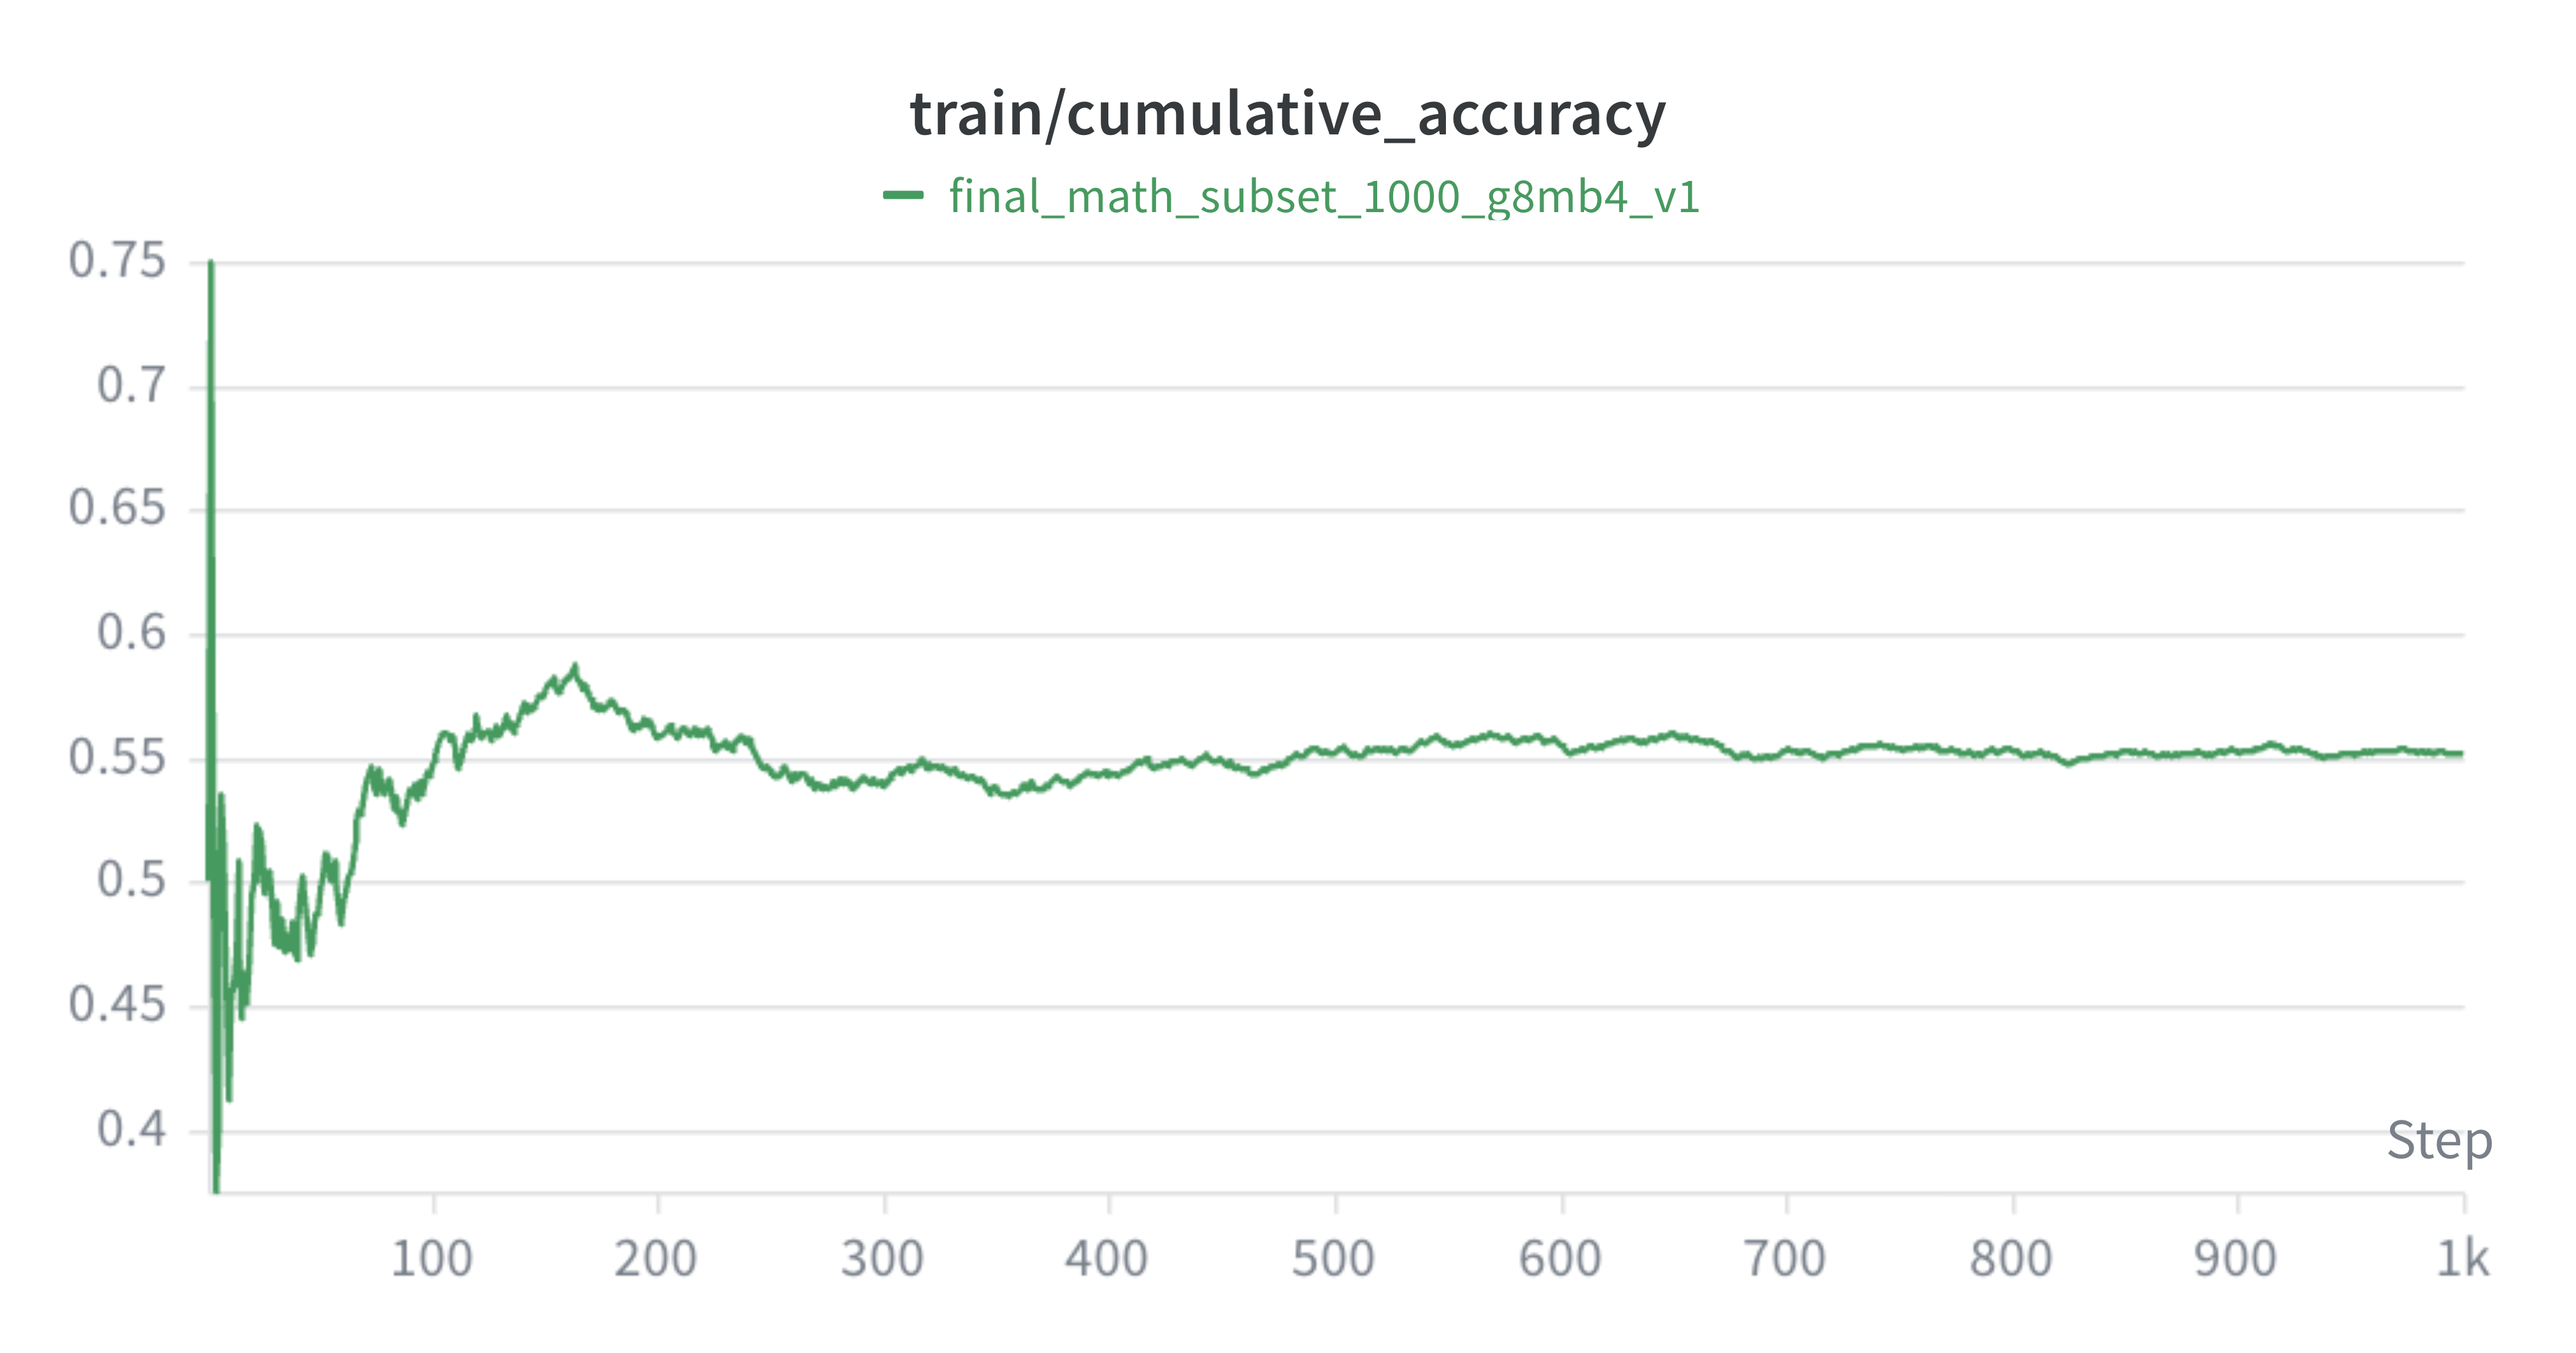
\includegraphics[width=\linewidth]{math_train_cumulative_accuracy.png}
    \caption{Cumulative training accuracy.}
  \end{subfigure}
  \hfill
  \begin{subfigure}{0.48\textwidth}
    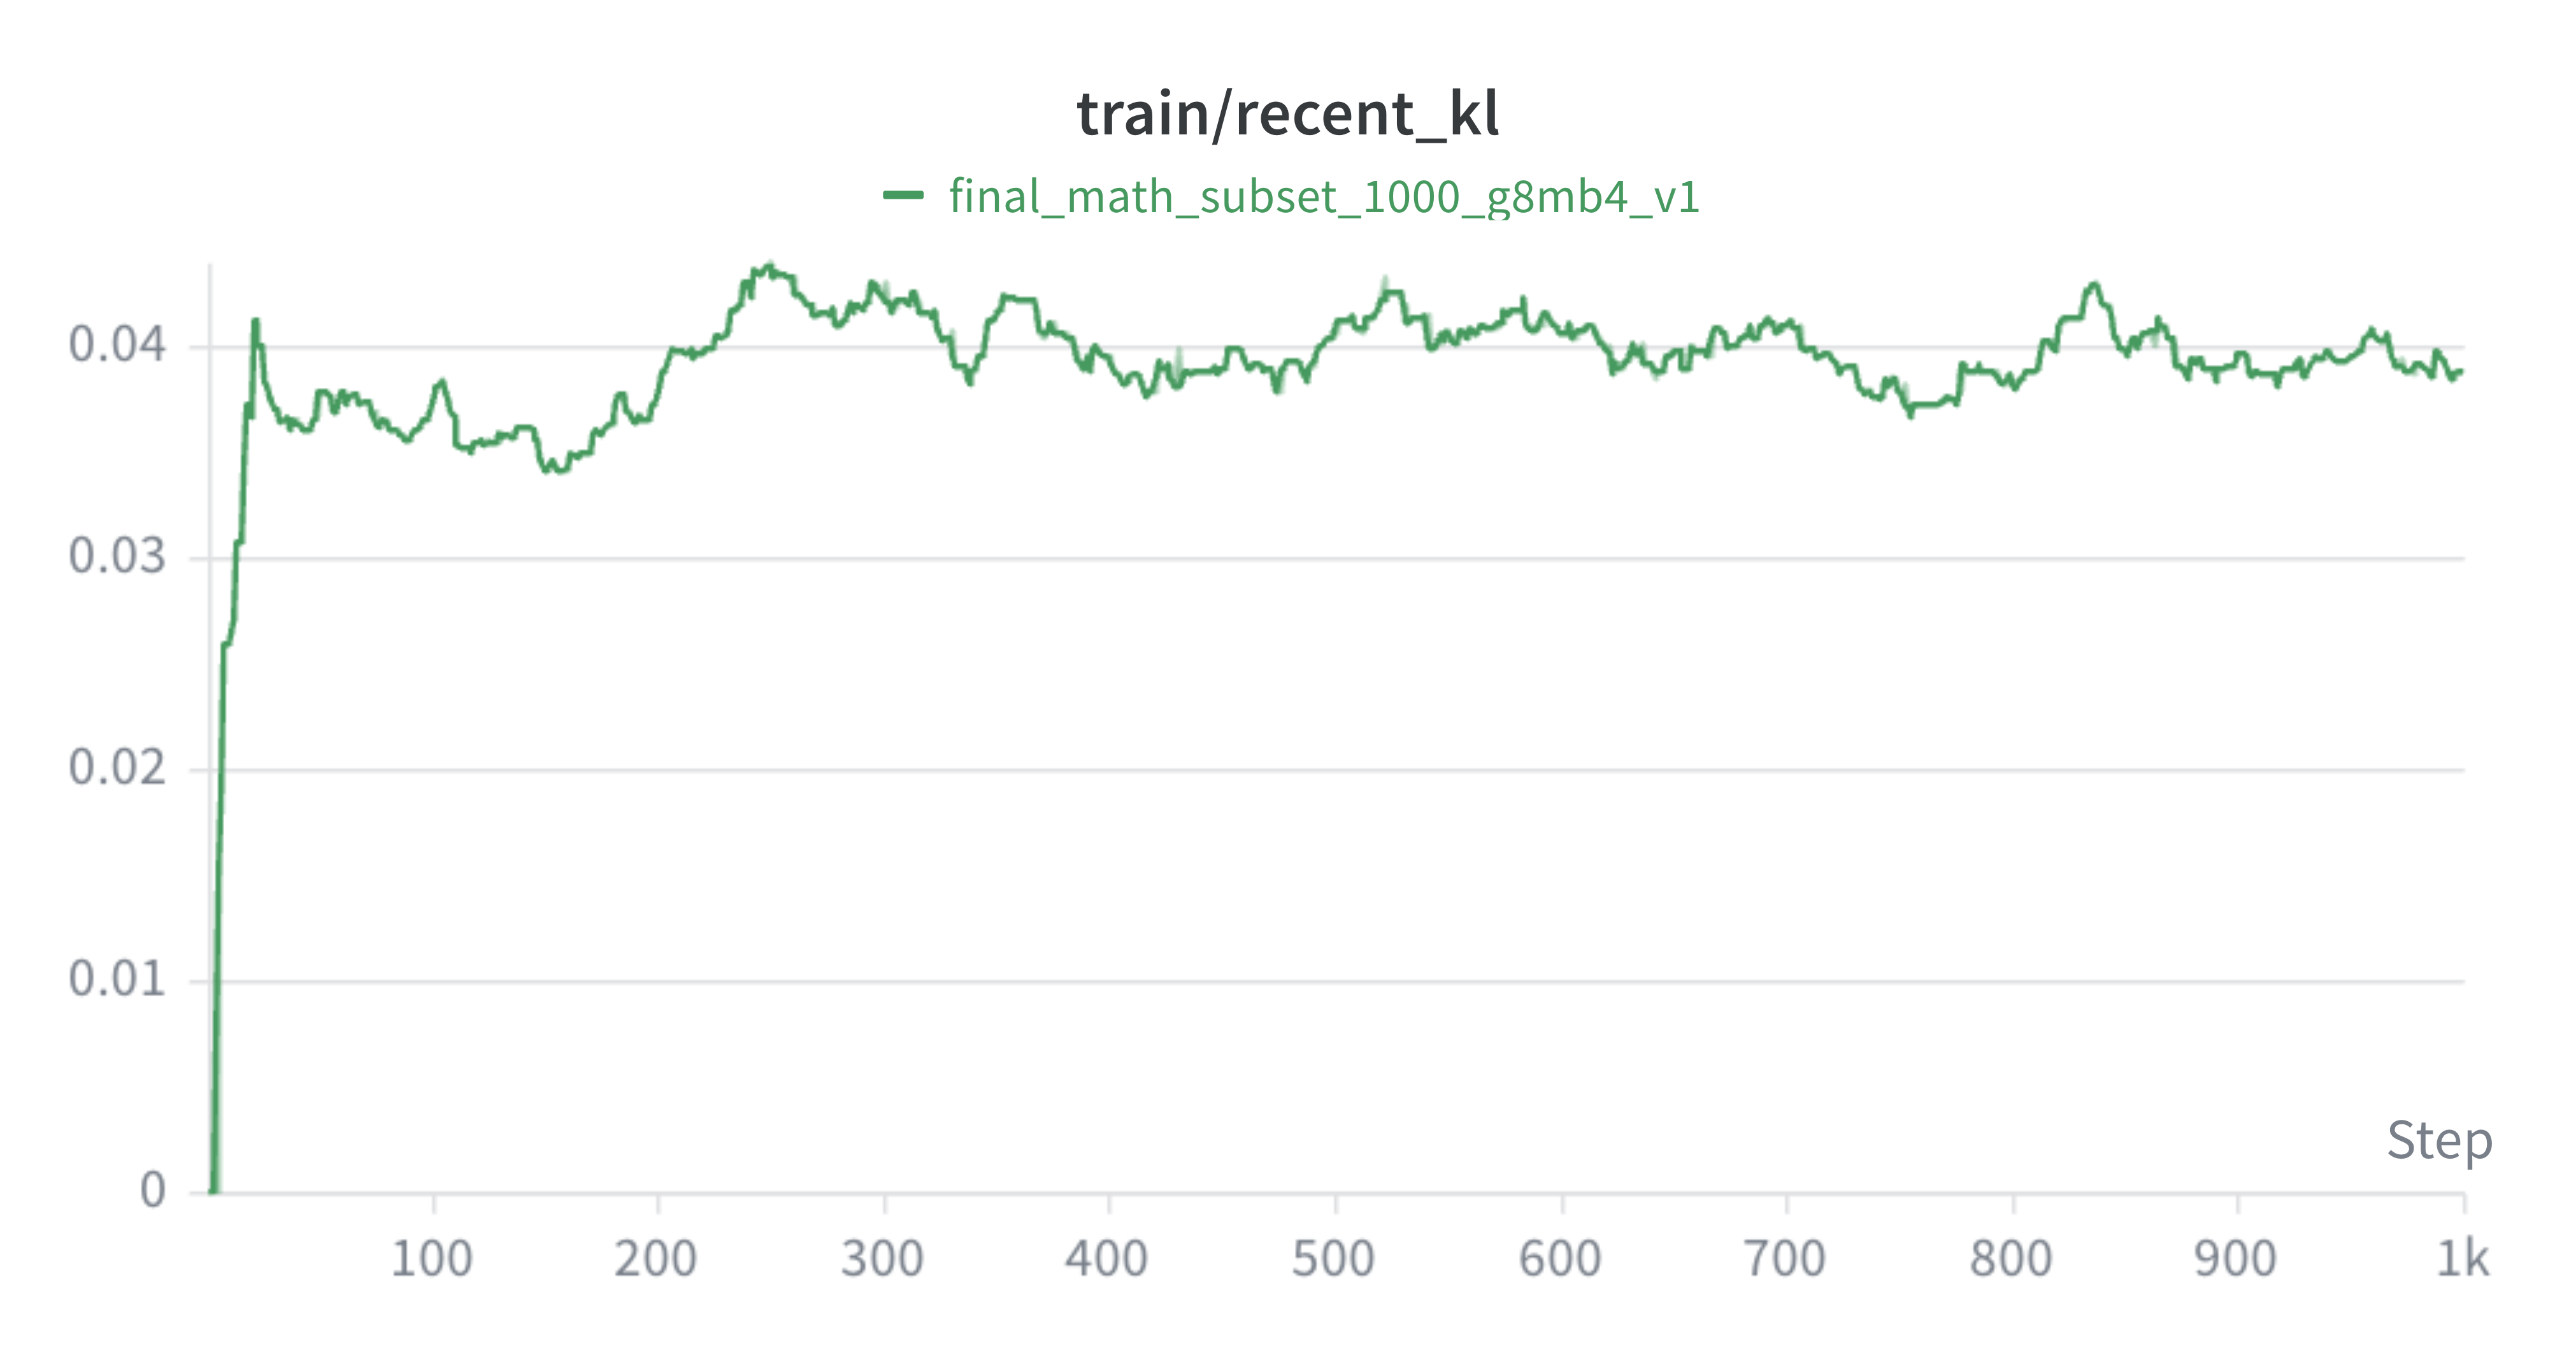
\includegraphics[width=\linewidth]{math_train_recent_kl.png}
    \caption{KL to the reference policy.}
  \end{subfigure}
  \caption{Training-time signals on the math-specialized base.}
  \label{fig:math-train}
\end{figure}

\paragraph{Test-set result.} On the full GSM8K test set, the post-training policy and the base model agree on correctness for $1{,}291/1{,}319 = 97.9\%$ of examples. Although they produce different reasoning traces for all problems, parameter updates lead to a symmetric effect where 14 examples flip from incorrect to correct and 14 from correct to incorrect, yielding no net change in accuracy.

\paragraph{Why the policy did not learn.}
GRPO produces gradients only when a group contains both successes and failures. All-correct and all-wrong groups yield zero advantage and only KL pressure. This leaves few informative groups because the base is already strong (about 85\% GSM8K accuracy at $T{=}0$), producing many all-correct groups even at $T{=}0.8$, while the remaining hard cases are mostly all-wrong. LoRA updates do not move the policy enough within the $0.04$ KL constraint.

\medskip
In contrast, Qwen2.5-1.5B-Instruct (general) trains successfully because its lower baseline accuracy yields more mixed-outcome groups. Our hypothesis is that the failure stems from insufficient gradient signal rather than a fundamental limitation of the base model.

\section{DAPO on the Math-Specialized Base}
\label{sec:dapo}

We address the bottlenecks identified in Section~\ref{sec:math-base} using DAPO-style dynamic group filtering \citep{yu2025dapo}, a larger LoRA, and a reduced KL penalty.

\paragraph{Setup.} The base model and prompt format are identical to Section~\ref{sec:math-base}. We increase LoRA rank from 8 to 32 and extend it to seven projection matrices, raising trainable parameters from $\sim$1.1M to $\sim$25M. The KL coefficient is reduced from 0.04 to 0.015.

\medskip
Training uses DAPO filtering with a target of 2 informative groups per step and up to 8 resampling attempts. We train on the \verb|mixed_hard| bucket ($\sim$1{,}738 examples) with $G{=}4$ rollouts per question and per-token normalization. Over training, 688 informative groups are retained from $\sim$1{,}738 sampled questions. Evaluation uses self-consistency with $K{=}8$ rollouts at $T{=}0.6$ and majority vote on the full GSM8K test set.

\paragraph{Training dynamics.}
Figure~\ref{fig:dapo-train} shows rolling accuracy and KL over 330 gradient steps. Compared to Figure~\ref{fig:math-train}, KL no longer pins and rises from near zero to $\sim$0.0008, remaining well below the 0.015 ceiling and indicating available optimization headroom.


\begin{figure}[h]
  \centering
  \begin{subfigure}{0.48\textwidth}
    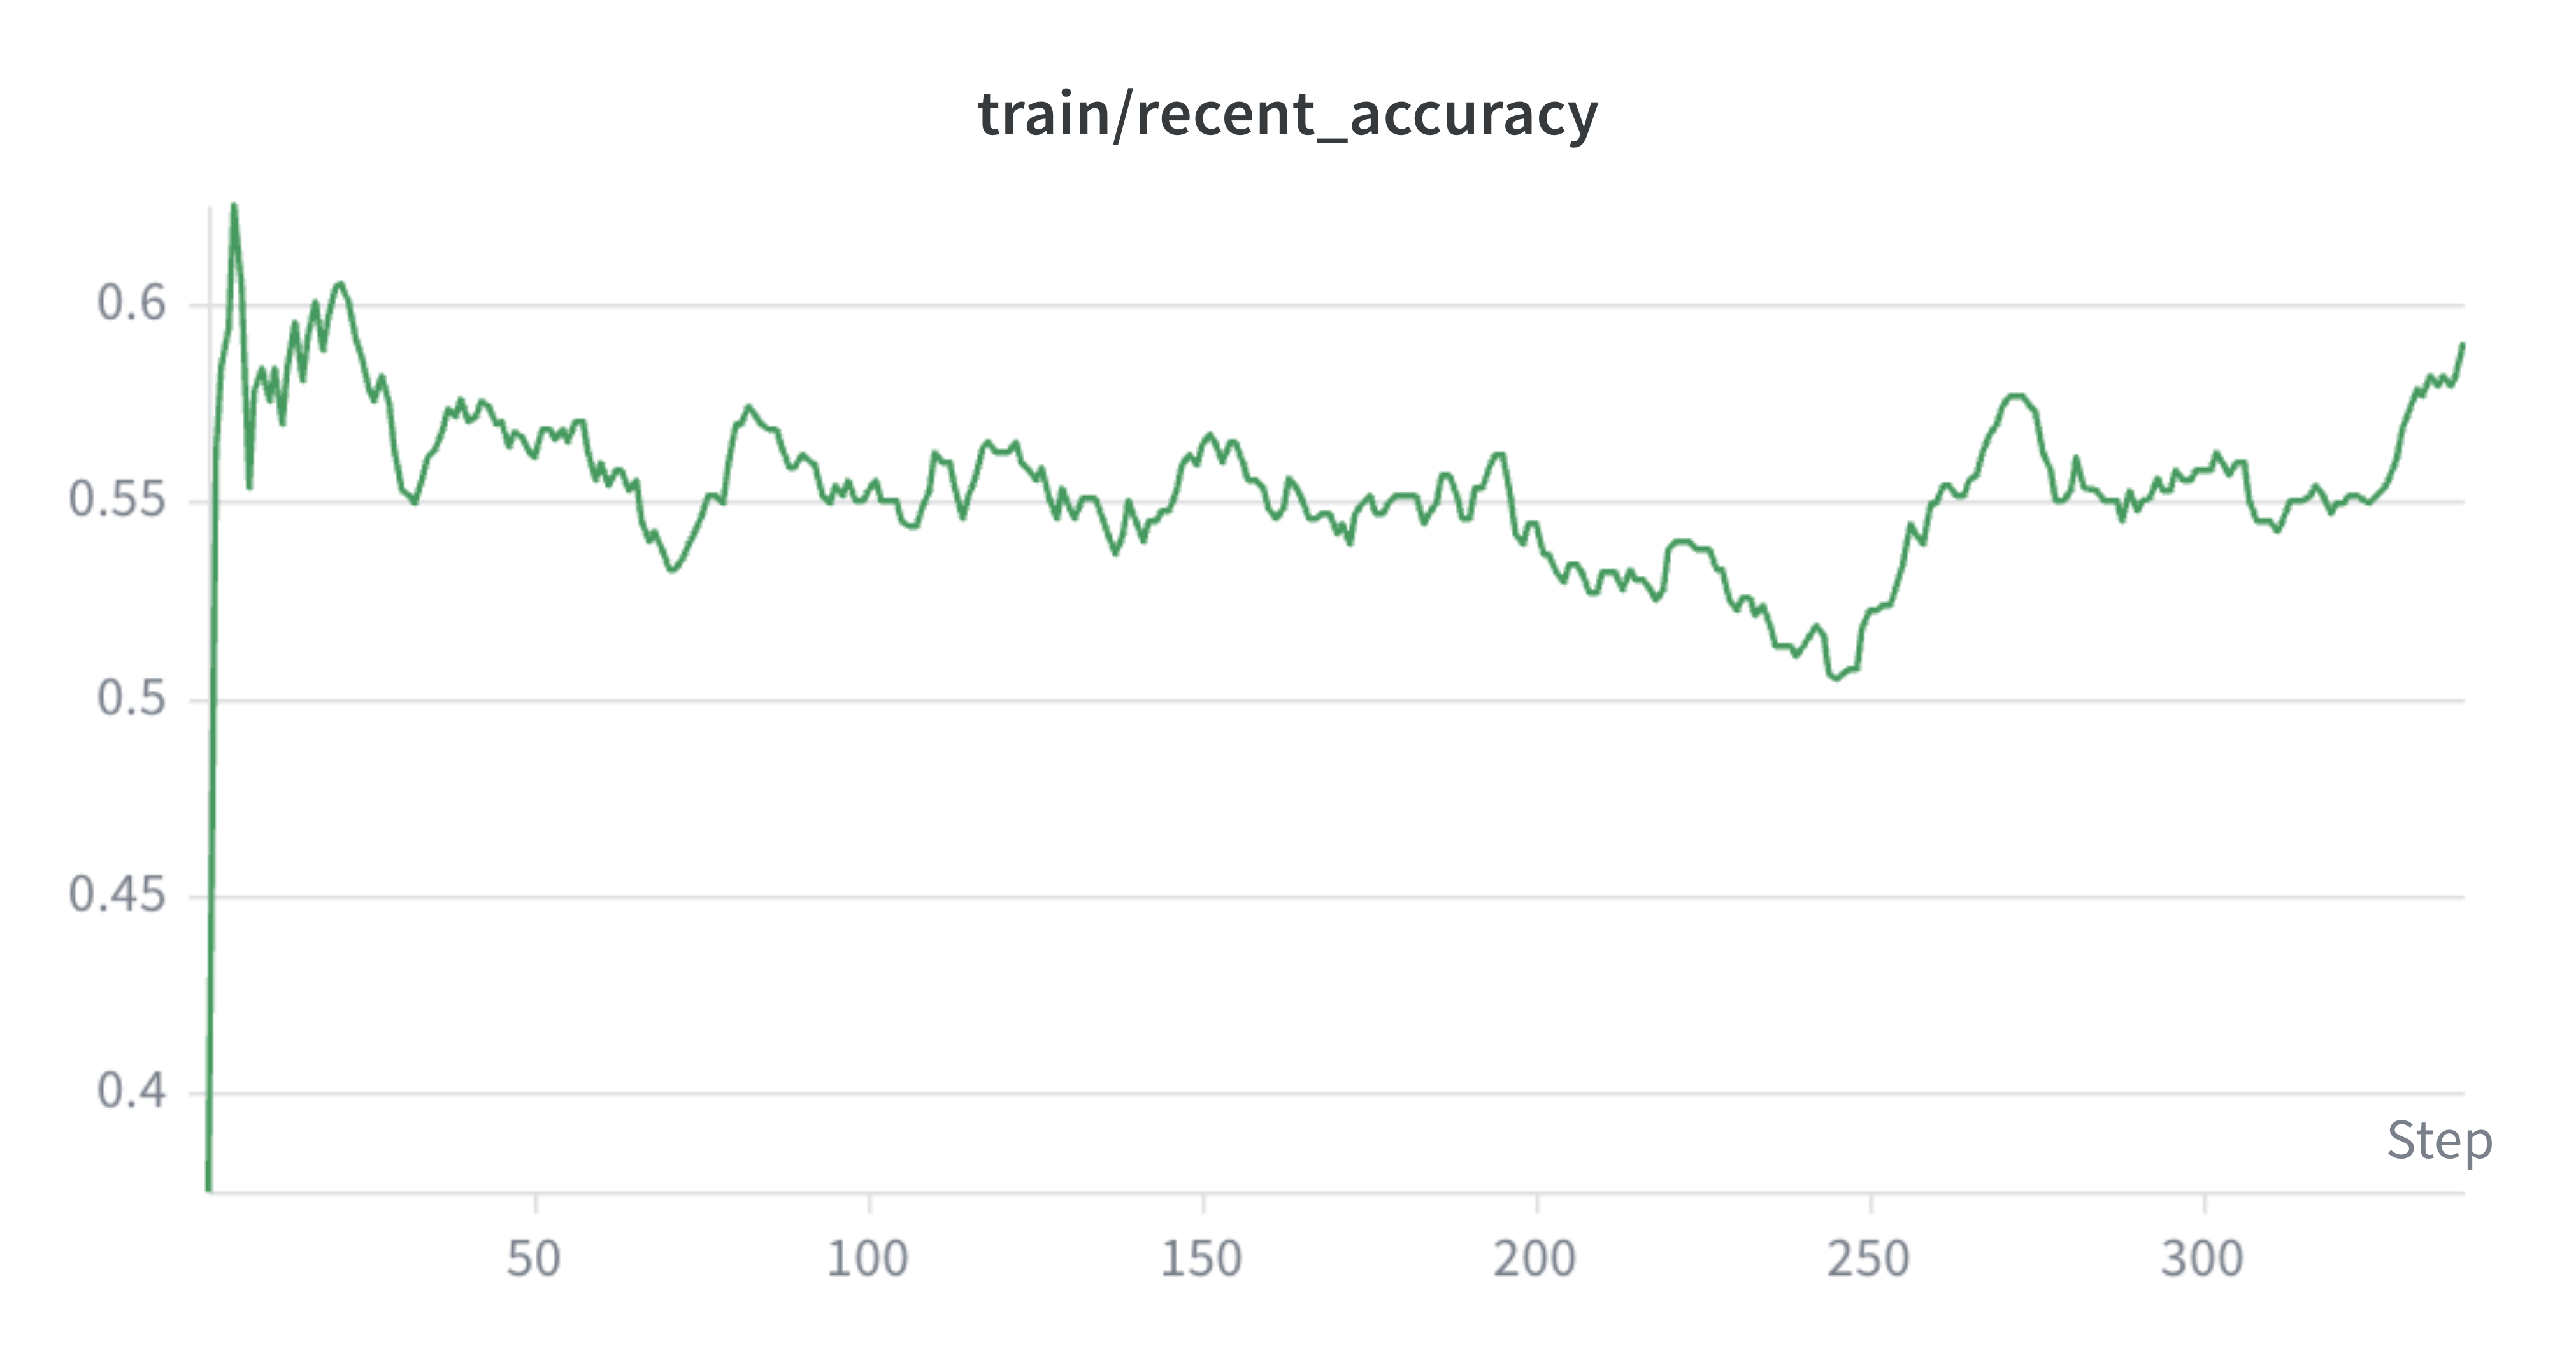
\includegraphics[width=\linewidth]{dapo_train_recent_accuracy.png}
    \caption{Rolling training accuracy}
  \end{subfigure}
  \hfill
  \begin{subfigure}{0.48\textwidth}
    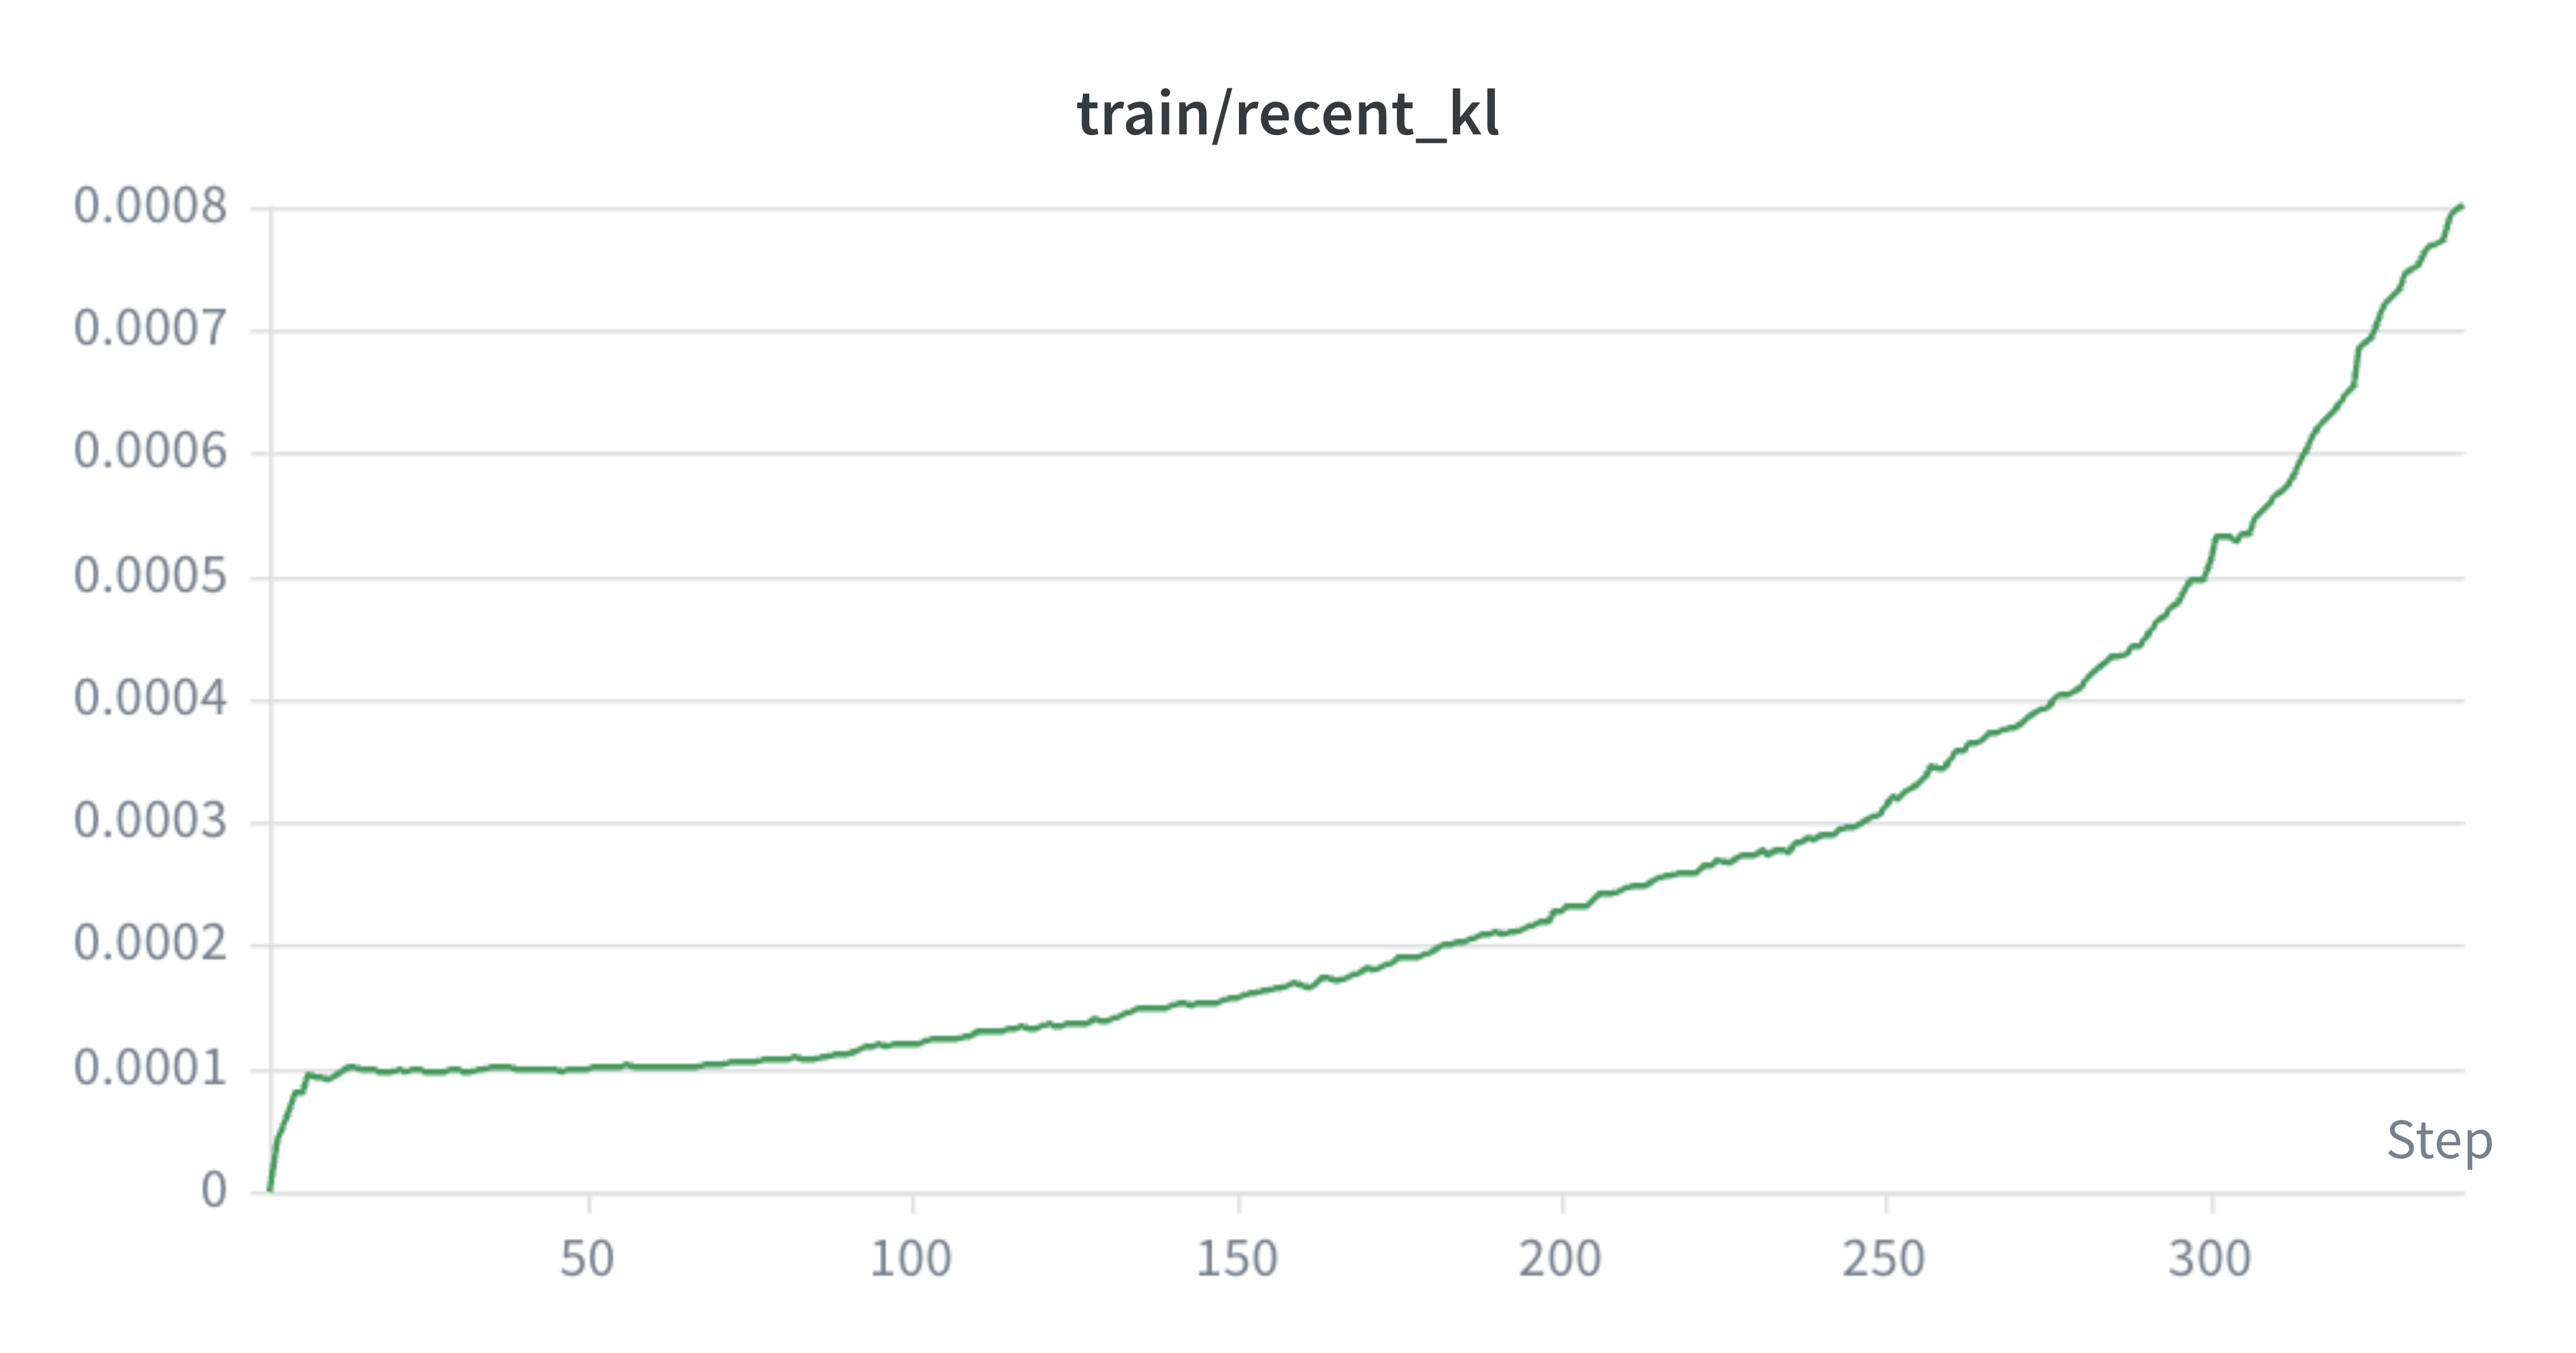
\includegraphics[width=\linewidth]{dapo_train_recent_kl.png}
    \caption{KL to the reference policy.}
  \end{subfigure}
  \caption{DAPO training dynamics on the math-specialized base ($\sim$330 gradient steps). \label{fig:dapo-train}}
\end{figure}

\paragraph{Test-set result.}
The DAPO-trained policy achieves $1{,}167/1{,}319 = 88.5\%$ majority-vote accuracy and $1{,}241/1{,}319 = 94.1\%$ pass@8 under $K{=}8$ self-consistency ($T{=}0.6$). The math base model yields $1{,}164/1{,}319 = 88.2\%$ majority-vote accuracy and $1{,}243/1{,}319 = 94.2\%$ pass@8 under the same protocol. The difference is $+3$ questions in majority-vote accuracy ($+0.3$ pp) and $-2$ in pass@8 ($-0.1$ pp), well within sampling noise. DAPO does not improve over the base.

\paragraph{Why training improved but test accuracy did not.}
Training diagnostics improve under DAPO. However, test accuracy does not improve because the math-specialized base already reaches 88.2\% under $K{=}8$ majority vote, and most remaining errors are all-wrong cases that DAPO explicitly filters out during training. As a result, there is effectively no gradient update signal on the hardest cases, and gains on borderline questions are too few to shift performance.

\section{Hierarchical Router--Solver Agent}
\label{sec:router-solver}

The negative result in Section~\ref{sec:math-base} motivated a different policy class. Instead of a single chain of thought, the agent decomposes the problem into an explicit \emph{plan} from a Router and a sequence of \emph{step executions} from a Solver, both LoRA adapters on a shared base. We built two versions. Neither closed the gap to the linear baselines, and the failure modes locate the bottleneck in the interface contract rather than in the base model's reasoning.

\subsection{V1: code-generating Solver with heuristic rewards}
\label{sec:rsv1}

V1 used one Qwen2.5-1.5B-Instruct base with two LoRA adapters. The Router emitted a numbered subgoal list, the Solver wrote a Python snippet per subgoal, and a sandboxed Python tool executed it. The outcome reward was binary on the final numeric answer; the only intermediate signal was a heuristic format and tool-call-success bonus. Training used GRPO over $B \cdot G$ trajectories per step, sharing one optimizer between the two adapters. V1 reached approximately $1.7\%$ test accuracy. Most of the engineering effort went into infrastructure, including vLLM memory pressure, sequential versus batched rollout, gradient checkpointing, and an out-of-memory fallback chunked backward path. The result was a $\sim$4$\times$ throughput improvement, $235$ to $58$ seconds per step at $B{=}2, G{=}4$, but no movement on test accuracy. The dominant failure mode was outcome-only credit assignment over a multi-step tool-using pipeline: a wrong final answer back-propagates negative gradient through every Router subgoal and every Solver snippet that produced it, whether or not each individual step was correct. The Python-tool contract added a second brittle interface, since Solver code that printed the right value but failed an answer-extraction regex still scored zero. At 1.5B with rank-8 LoRA, the joint policy did not have either the capacity or the signal-to-noise ratio to learn this contract from outcome reward alone.

\subsection{V2: text-reasoning Solver with judge-based dense rewards}
\label{sec:rsv2}

\paragraph{Setup.} V2 replaced the Python Solver with a text-reasoning Solver and added a remote judge (GPT-4o-mini) that scored three quantities per rollout: a plan reward from the Router's JSON plan, a step-level reward for each Solver step, and a binary outcome reward on the final answer. GRPO then operated on a weighted advantage combining router, step, and outcome contributions, with the router weight decaying 5\% per epoch and the outcome weight increasing correspondingly. Judging was batched ten items per API call, bringing inference cost from $\sim$\$75 to $\sim$\$10 per full pass. Training used $G{=}4$ rollouts over $7{,}500$ questions for one epoch, roughly $30{,}000$ rollouts.

\paragraph{Result.} On a 20-question traced sample, raw rollout accuracy was 10.8\%. The best inference-side intervention, an answer-synthesis step that re-prompts the Solver with the full trajectory and asks for a single final number, lifted that to 20.0\%. A larger fresh-eval pass on the trained checkpoint reached about 35\% rollout accuracy with synthesis on. This is well above V1's 1.7\% but still about 50 points below the 71.6\% greedy accuracy of the linear RLVR policy (Section~\ref{sec:linear}).

\paragraph{Why V2 did not work.} Rather than guess, we built a per-rollout failure taxonomy on the traced $20\mathrm{Q} \times G{=}6$ sample and counted bucket frequencies. About 51.7\% of failed rollouts are not core reasoning failures but architectural failures of the Router--Solver contract: \texttt{copied\_intermediate\_as\_final} (15.8\%, the emitted final answer matches an earlier intermediate quantity), \texttt{correct\_number\_in\_trace\_wrong\_final} (12.5\%, the correct number appears in the rollout text but extraction picks a different number), \texttt{plan\_endpoint\_mismatch} (10.0\%, the last subgoal is not the global answer target), and \texttt{plan\_parse\_failed} (13.3\%, Router JSON does not parse). Only 37.5\% of failures were \texttt{wrong\_numeric\_final}, the Solver actually computing the wrong number. V2's ceiling is set by structural choices (last step equals final answer, JSON-parseable plans, outcome credit attached only to the last step's log-probs), not by an inability of the base to do grade-school arithmetic.

\paragraph{Attempted fixes that did not generalize.} Two interventions were tested directly. Router prompt hardening, a stricter template intended to drive \texttt{plan\_parse\_failed} to zero, caused a catastrophic regression on an isolated 10Q split (20.0\% to 3.3\% with only $9/60$ valid rollouts), because the harder prompt made the Router refuse to emit plans on out-of-template questions. Outcome credit on all steps, a training-side change that distributes the outcome reward across every Solver step's log-probs, improved in-loop training accuracy (15.0\% to 26.7\%) but lost on a fresh traced eval (35.0\% to 28.3\%): the variant overfit to sampled training trajectories and produced a weaker policy on fresh draws. The inference-side fix that did help, final-answer synthesis, works precisely because it bypasses the last-step-equals-final-answer assumption that the taxonomy identified as the largest single failure source.

\paragraph{Reading.} V2 is bottlenecked by the Router--Solver interface design, not by reasoning capability at this scale. The question-level taxonomy shows 25\% of questions already have at least one correct rollout in their $G{=}6$ group, with a projected 90\% if all non-core failures were eliminated. The base model produces usable reasoning often enough that the actual bottleneck is whether the system can extract a single correct scalar from a multi-step trajectory. At 1.5B with rank-8 LoRA, an outcome-only or step-judged reward cannot supervise that contract into shape. The next architectural change has to flatten or supervise the Router--Solver hand-offs rather than just decompose harder, which is the motivation for the graph-memory and hierarchical-RL extensions in the larger project plan.

\subsection{V3: three-branch hierarchical pivot}
\label{sec:rsv3}

\paragraph{Setup.} V3 takes V2's failure taxonomy seriously and changes the interface before changing the optimizer. The system now exposes three execution branches: \emph{easy}, a cheap single-pass chain-of-thought path; \emph{soft}, the main hierarchical Router--Solver branch; and \emph{hard}, the same hierarchical branch augmented with retrieval from a Hopfield-style graph memory of solved cases. The current production candidate is \emph{soft}, not \emph{hard}. Its frozen contract removes global answer synthesis, keeps plan-parse repair on, turns router hardening and strict answer-format heuristics off, repairs the last subgoal so it is answer-bearing, and returns the deterministic majority vote over rollout-local final answers. The headline diagnostic uses a fixed $10$-question slice with $G{=}6$ rollouts per question; the best known setting is \texttt{solver\_temperature=0.7}.

\paragraph{Result.} On that fixed $10\mathrm{Q}\times G{=}6$ diagnostic contract, the \emph{soft} branch reaches $0.90$ question-majority relaxed accuracy, $1.00$ question-any relaxed accuracy, and $0.4833$ rollout relaxed accuracy ($29/60$ correct rollouts). This is the strongest hierarchical result in the repo and a substantial improvement over V2's $\sim$35\% rollout accuracy. The gain comes from simplifying the answer contract rather than from a stronger RL recipe: the branch no longer asks the model to synthesize one global answer after a long trajectory, and instead votes over local final answers that are explicitly tied to answer-bearing last steps. At the same time, the result is not yet directly comparable to the linear baselines (Section~\ref{sec:linear}), because the clean \emph{soft}-only and oracle-routed evaluations beyond the fixed diagnostic slice are still pending.

\paragraph{What improved and what did not.} The central V2 failure mode was that the model often computed the right scalar somewhere in the trace but lost answer identity at the final hand-off. V3 reduces that failure materially, but it does not eliminate it. Across the traced V3 ablations, the dominant residual category is still \texttt{correct\_number\_in\_trace\_wrong\_final}; for example, an answer-bearing-hardened 10Q trace logged $29$ such failures versus only $7$ pure \texttt{wrong\_numeric\_final} errors. The current read is therefore unchanged at a deeper level: the base can often do the arithmetic, but the hierarchy still corrupts the answer target at the endpoint.

\paragraph{Reading.} V3 changes the conclusion from ``hierarchy does not work'' to ``hierarchy only helps when the contract is simplified aggressively.'' The \emph{soft} branch is now real enough to justify branch-separation and supervised-routing work, while the \emph{hard} retrieval branch remains research-only. Just as importantly, porting the stronger DAPO discipline into the hierarchy did not rescue training: a minimal informative-group-sampling + all-steps-credit port regressed to $0.30$ question-majority accuracy on the corrected 10Q/$G{=}5$ eval. That negative result reinforces the main diagnosis from V2. The next gain is more likely to come from branch routing and interface supervision than from another local tweak to the hierarchical GRPO trainer.

\section{Conclusion and Future Work}
\label{sec:conclusion}

Four experiments on GSM8K at the 1.5B scale yield a consistent picture. Vanilla LoRA-GRPO succeeds only when the base model produces enough mixed-outcome groups for GRPO to generate signal, which holds for the general base ($\sim$70\% greedy) but not the math-specialized base ($\sim$85\% greedy), where a dead-gradient regime appears immediately. DAPO with dynamic group filtering, wider LoRA, and a reduced KL budget fixes training dynamics: KL no longer pins and reward increases steadily. However, test performance does not move meaningfully; the math base already achieves 88.2\% majority-vote accuracy, and DAPO reaches 88.5\%, a three-question difference within noise. The hierarchical Router--Solver agent also fails, not due to reasoning limits of the base model, but because the interface contract cannot be learned from outcome reward alone at this scale, with 51.7\% of failures being architectural rather than numeric.

Future work follows directly. On the RL side, isolating DAPO components (group filtering, LoRA rank, KL coefficient) and reporting greedy evaluation on the same footing as baselines would clarify which factors matter. On the agent side, the Router--Solver interface likely requires direct supervision, either by collapsing into a single-model scratchpad or adding a lightweight verifier for plan-step consistency. Longer-horizon extensions such as graph-memory retrieval and hierarchical RL with explicit subgoal rewards remain open once the single-step interface is stabilized.

\newpage
\appendix
\begin{center}
  {\large\textbf{Appendix}}
\end{center}
\vspace{0.5em}

\section{Hardware and Compute}
\label{app:hardware}

All training runs were executed on a single NVIDIA L4 GPU (24\,GB VRAM). The software stack is PyTorch with HuggingFace \texttt{transformers} and \texttt{peft} for LoRA adaptation. The DAPO run initially used vLLM for rollout generation but fell back to HF generation due to memory constraints from model replication during inference. Table~\ref{tab:compute} summarizes rollout counts and approximate wall-clock times per experiment.

\begin{table}[h]
  \centering
  \begin{tabular}{lrrl}
    \toprule
    Experiment & Questions & Total rollouts & Wall-clock \\
    \midrule
    Linear GRPO (general base)  & 2{,}000  & 12{,}000          & $\sim$7\,h \\
    GRPO on math base           & 1{,}000  & 8{,}000           & $\sim$7\,h \\
    DAPO on math base           & 1{,}738\textsuperscript{$\dagger$} & $\sim$7{,}000 & $\sim$8\,h \\
    Router--Solver V2           & 7{,}500  & 30{,}000          & $\sim$40\,h\textsuperscript{$\ddagger$} \\
    \bottomrule
  \end{tabular}
  \caption{Compute summary. All runs on a single NVIDIA L4 (24\,GB). \textsuperscript{$\dagger$}Questions attempted before DAPO group filtering; 688 informative groups were kept. \textsuperscript{$\ddagger$}Includes latency from batched GPT-4o-mini judge API calls.}
  \label{tab:compute}
\end{table}

\section{Additional Training Curves}
\label{app:curves}

This appendix collects the training signals not included in the main figures: per-step reward and policy loss for all three RL experiments, and the remaining accuracy curves omitted for space.

\subsection{Linear GRPO on the General Base}
\label{app:linear}

\begin{figure}[H]
  \centering
  \begin{subfigure}{0.32\textwidth}
    
\includegraphics[width=\linewidth]{train_recent_reward.png}
    \caption{Rolling reward.}
  \end{subfigure}
  \hfill
  \begin{subfigure}{0.32\textwidth}
    
\includegraphics[width=\linewidth]{train_recent_loss.png}
    \caption{Policy loss.}
  \end{subfigure}
  \hfill
  \begin{subfigure}{0.32\textwidth}
    
\includegraphics[width=\linewidth]{train_recent_kl.png}
    \caption{KL to reference.}
  \end{subfigure}
  \caption{Additional training signals for the linear GRPO run on Qwen2.5-1.5B-Instruct (Section~\ref{sec:linear}). Per-rollout reward climbs from $\sim$1.1 to $\sim$1.3 (out of a 1.5 ceiling); policy loss stays cleanly negative; KL grows monotonically but remains bounded by the 0.04 penalty.}
  \label{fig:app-linear}
\end{figure}

\subsection{GRPO on the Math-Specialized Base}
\label{app:math}

\begin{figure}[H]
  \centering
  \begin{subfigure}{0.32\textwidth}
    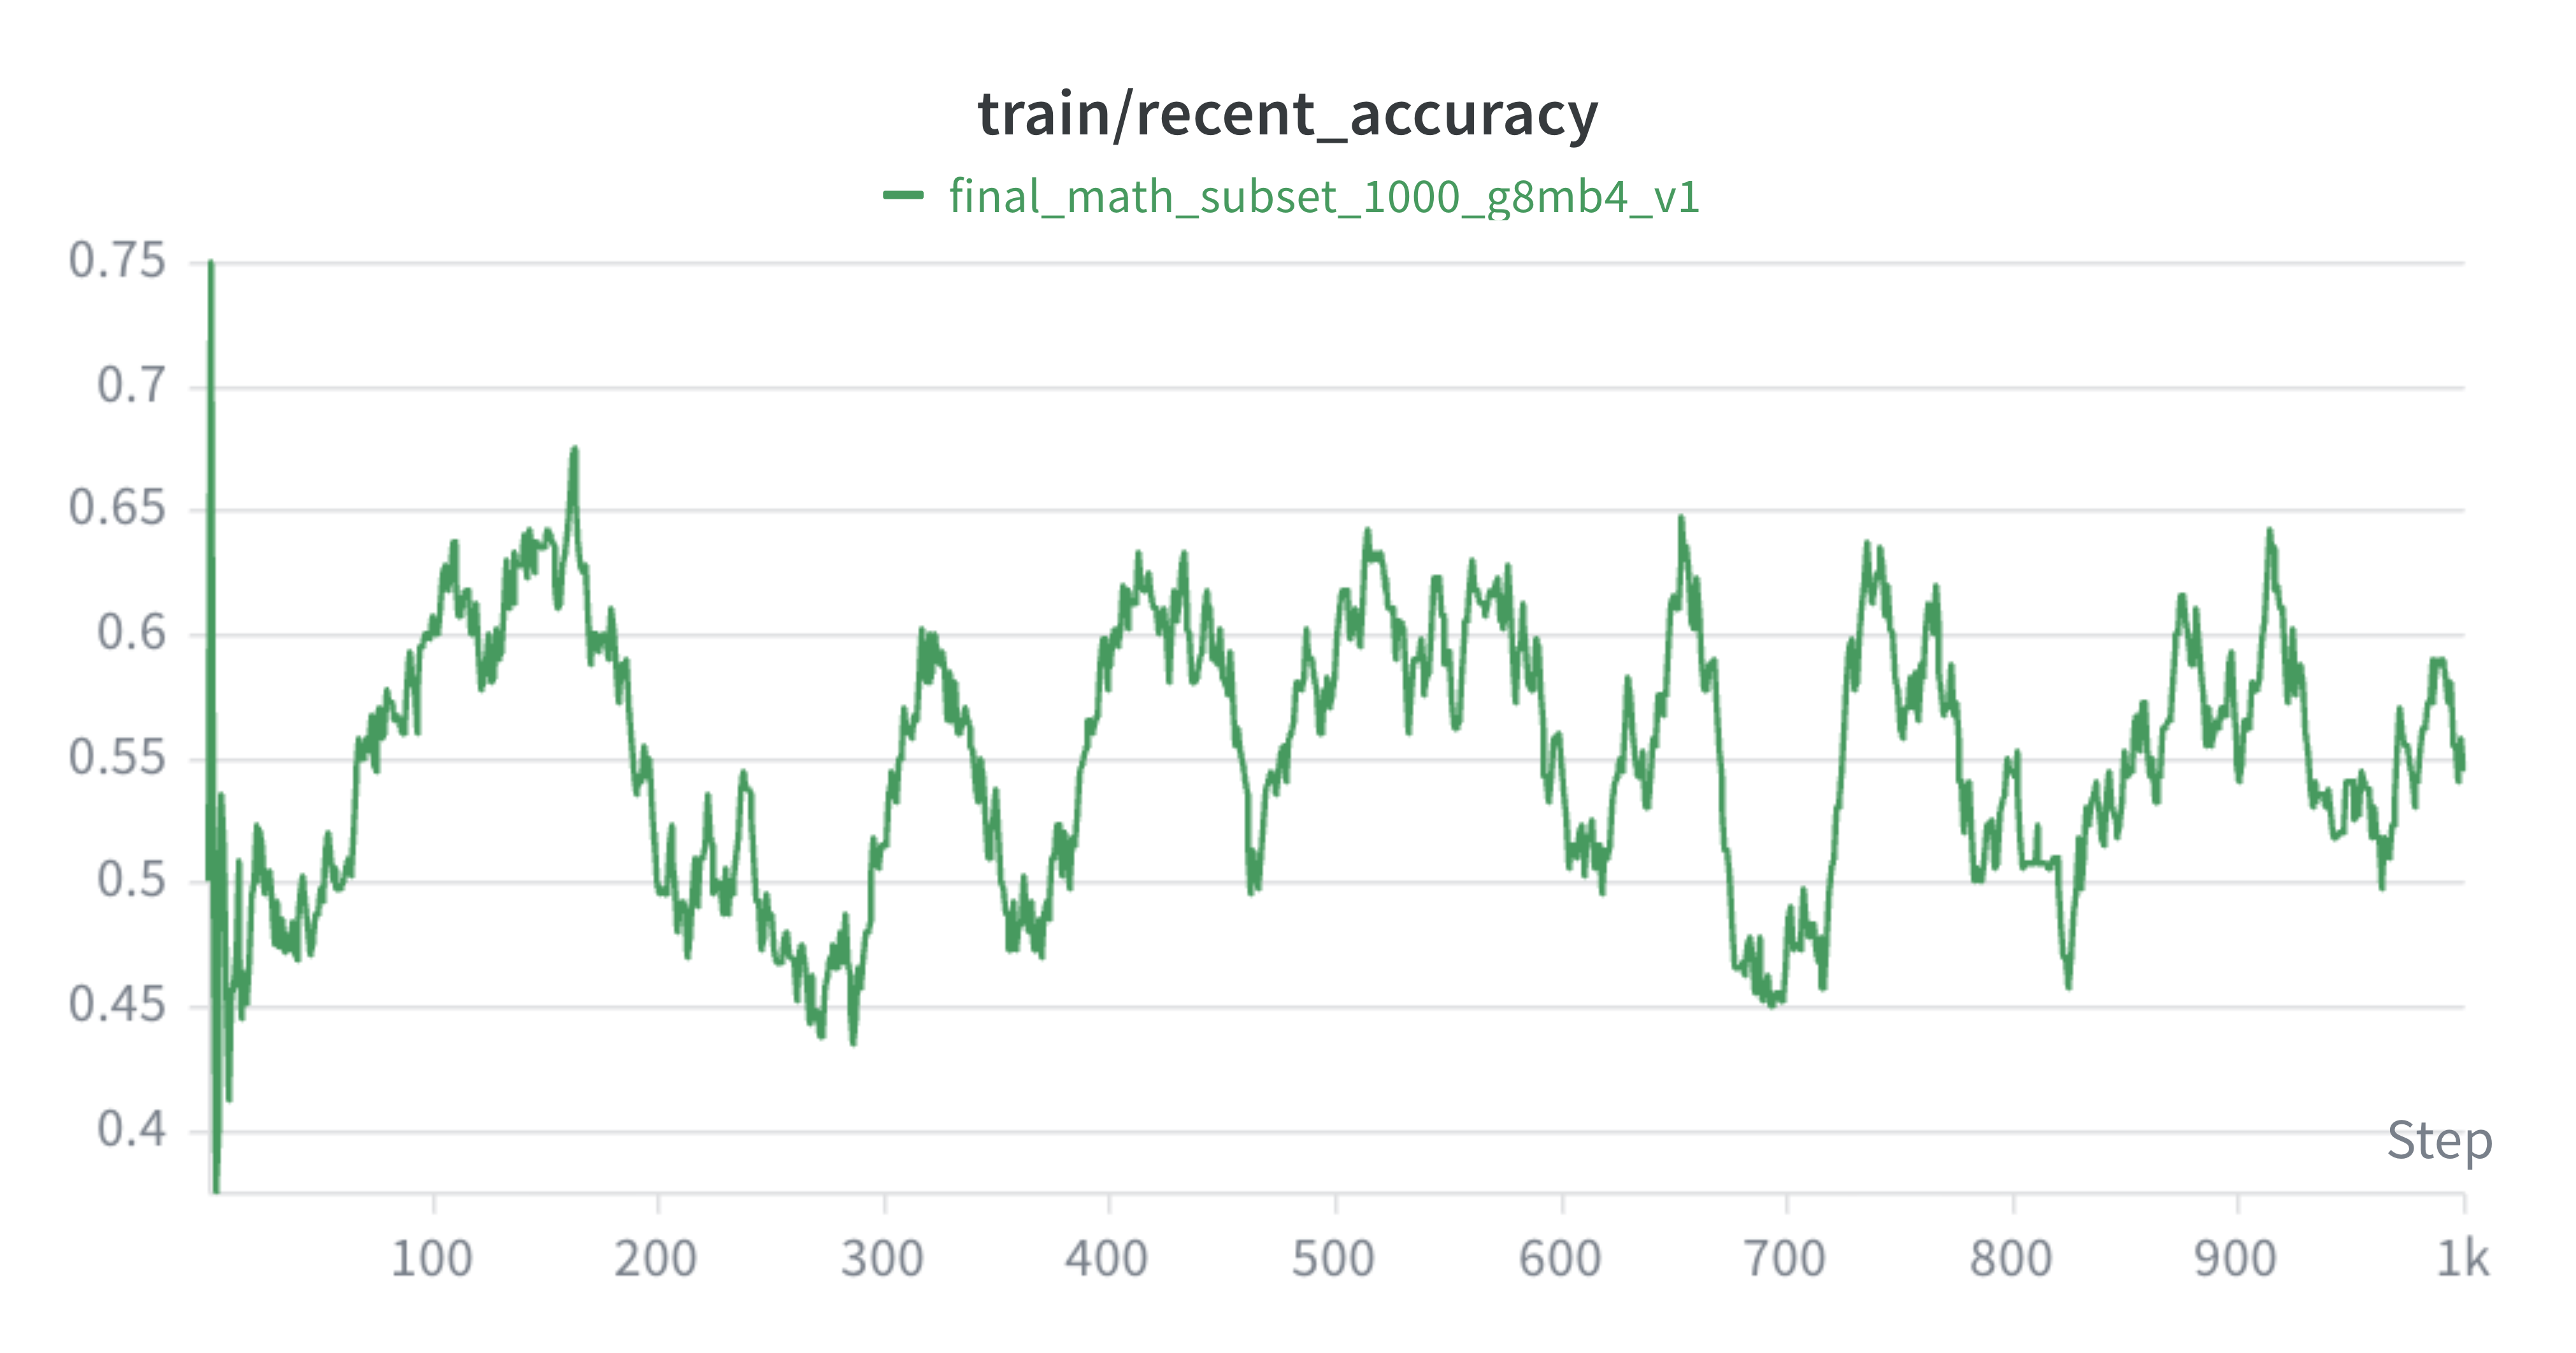
\includegraphics[width=\linewidth]{math_train_recent_accuracy.png}
    \caption{Rolling accuracy.}
  \end{subfigure}
  \hfill
  \begin{subfigure}{0.32\textwidth}
    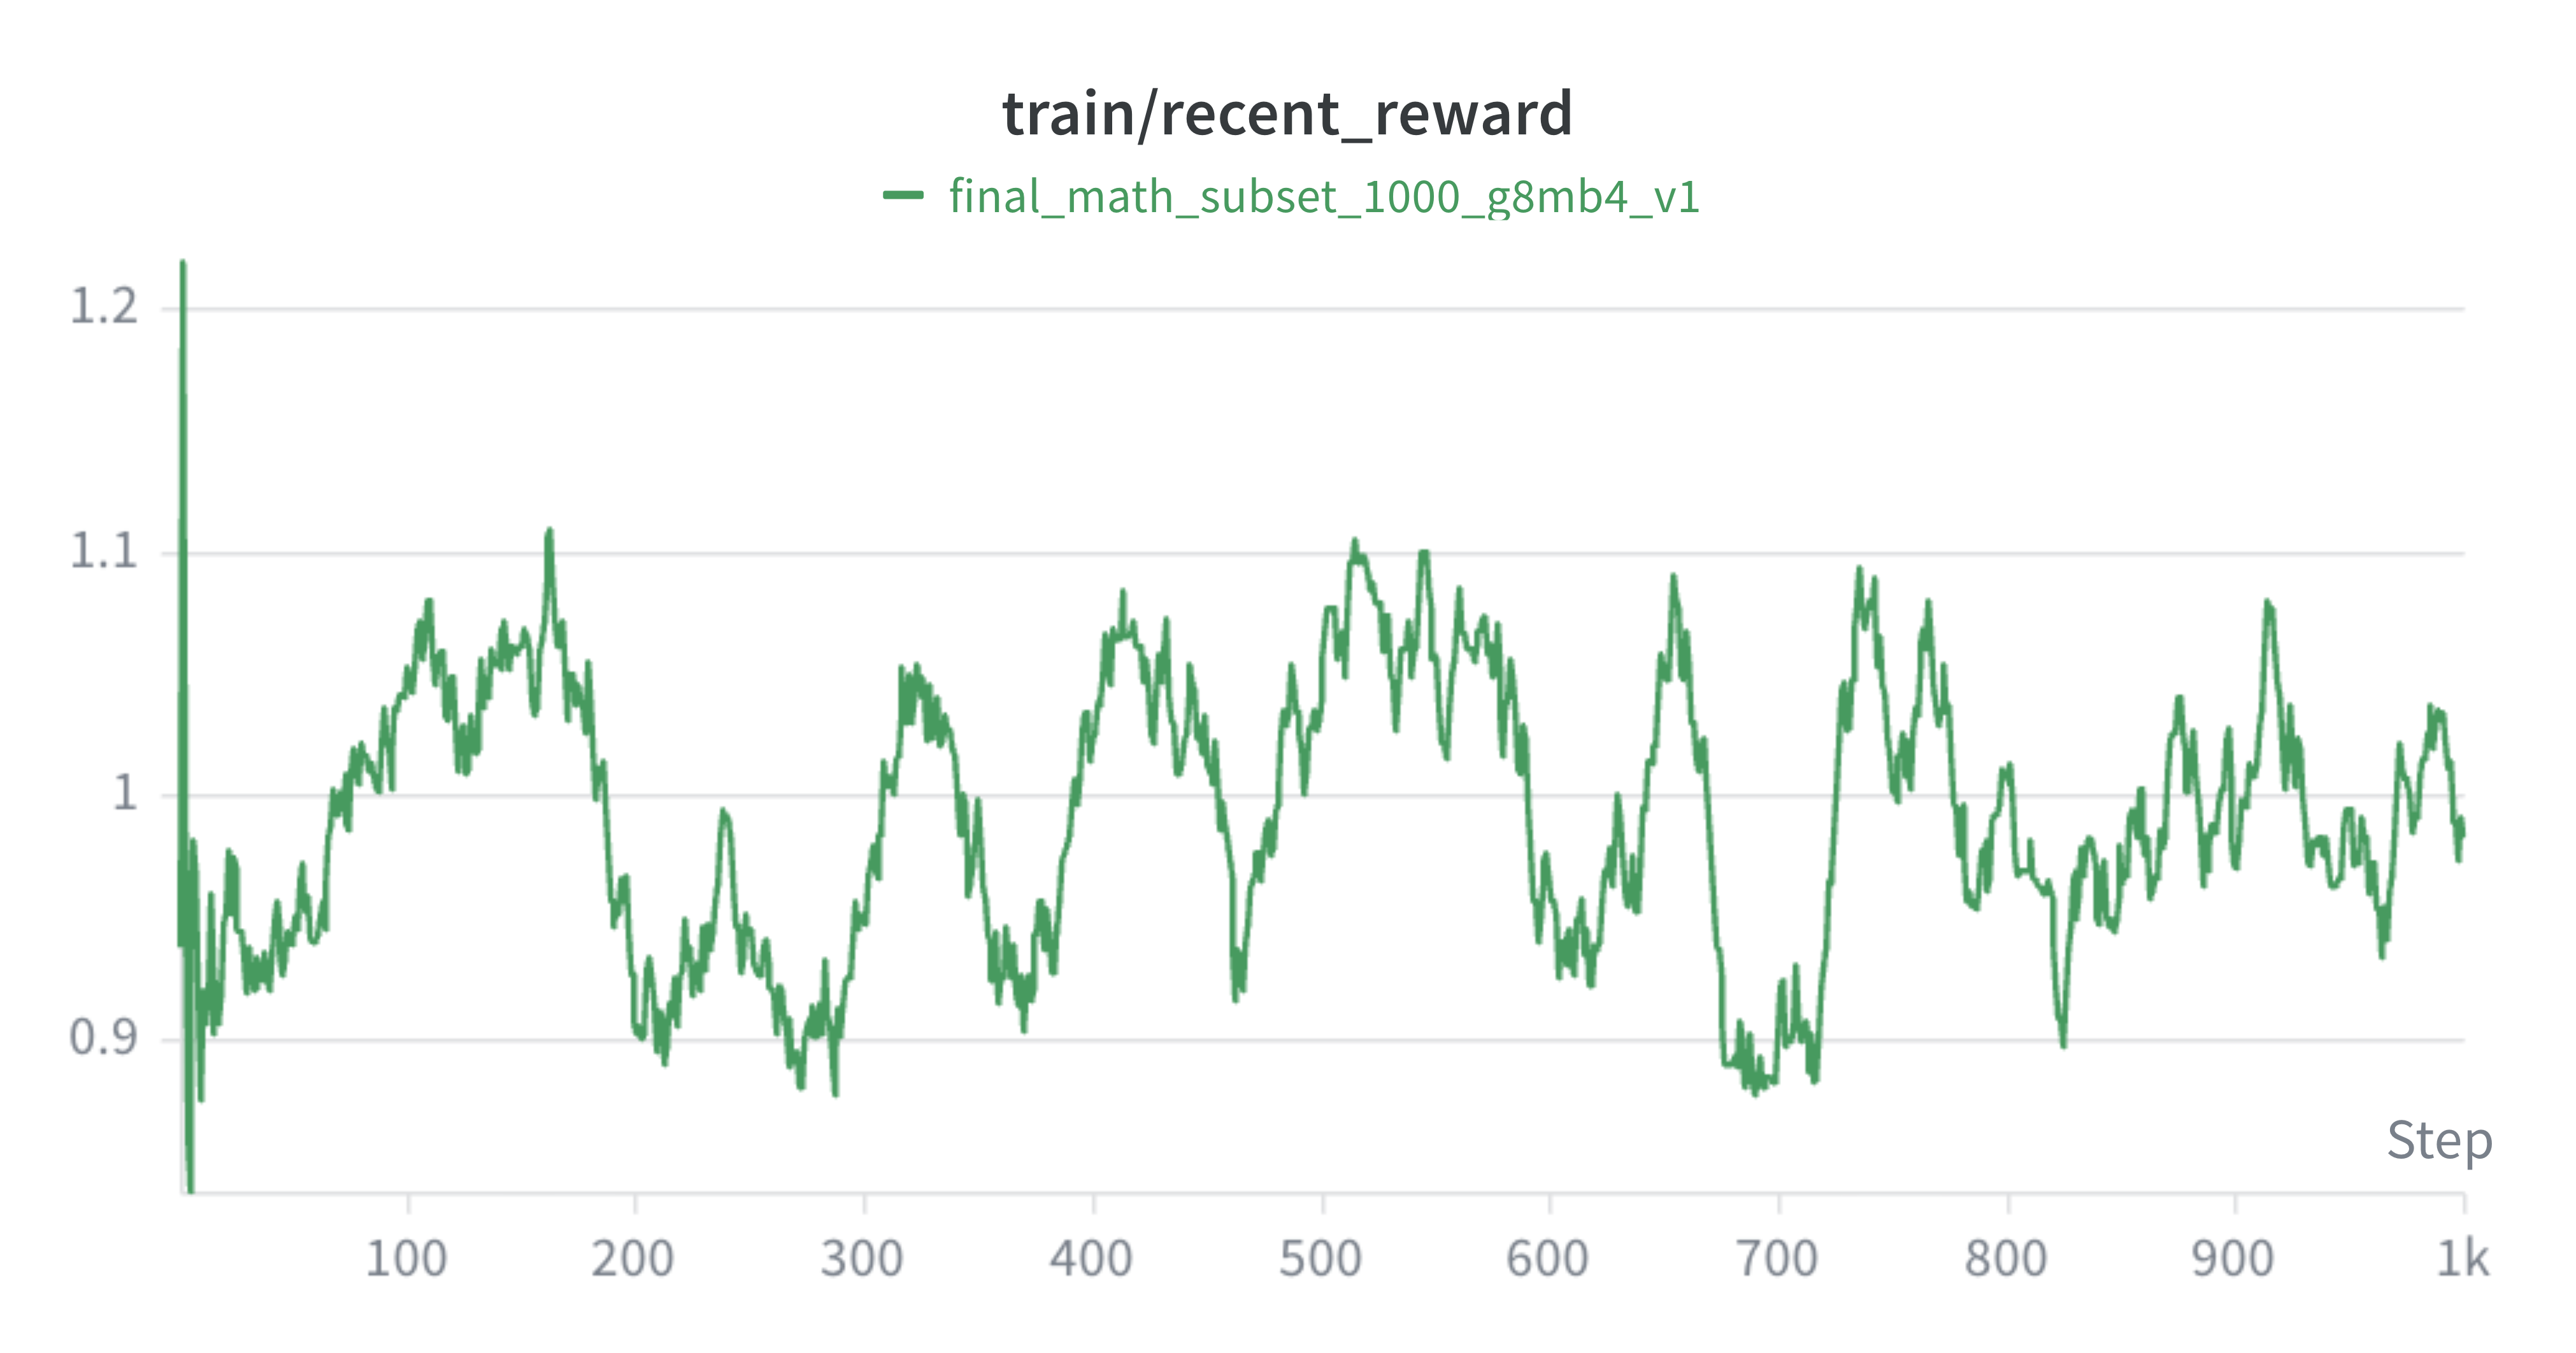
\includegraphics[width=\linewidth]{math_train_recent_reward.png}
    \caption{Rolling reward.}
  \end{subfigure}
  \hfill
  \begin{subfigure}{0.32\textwidth}
    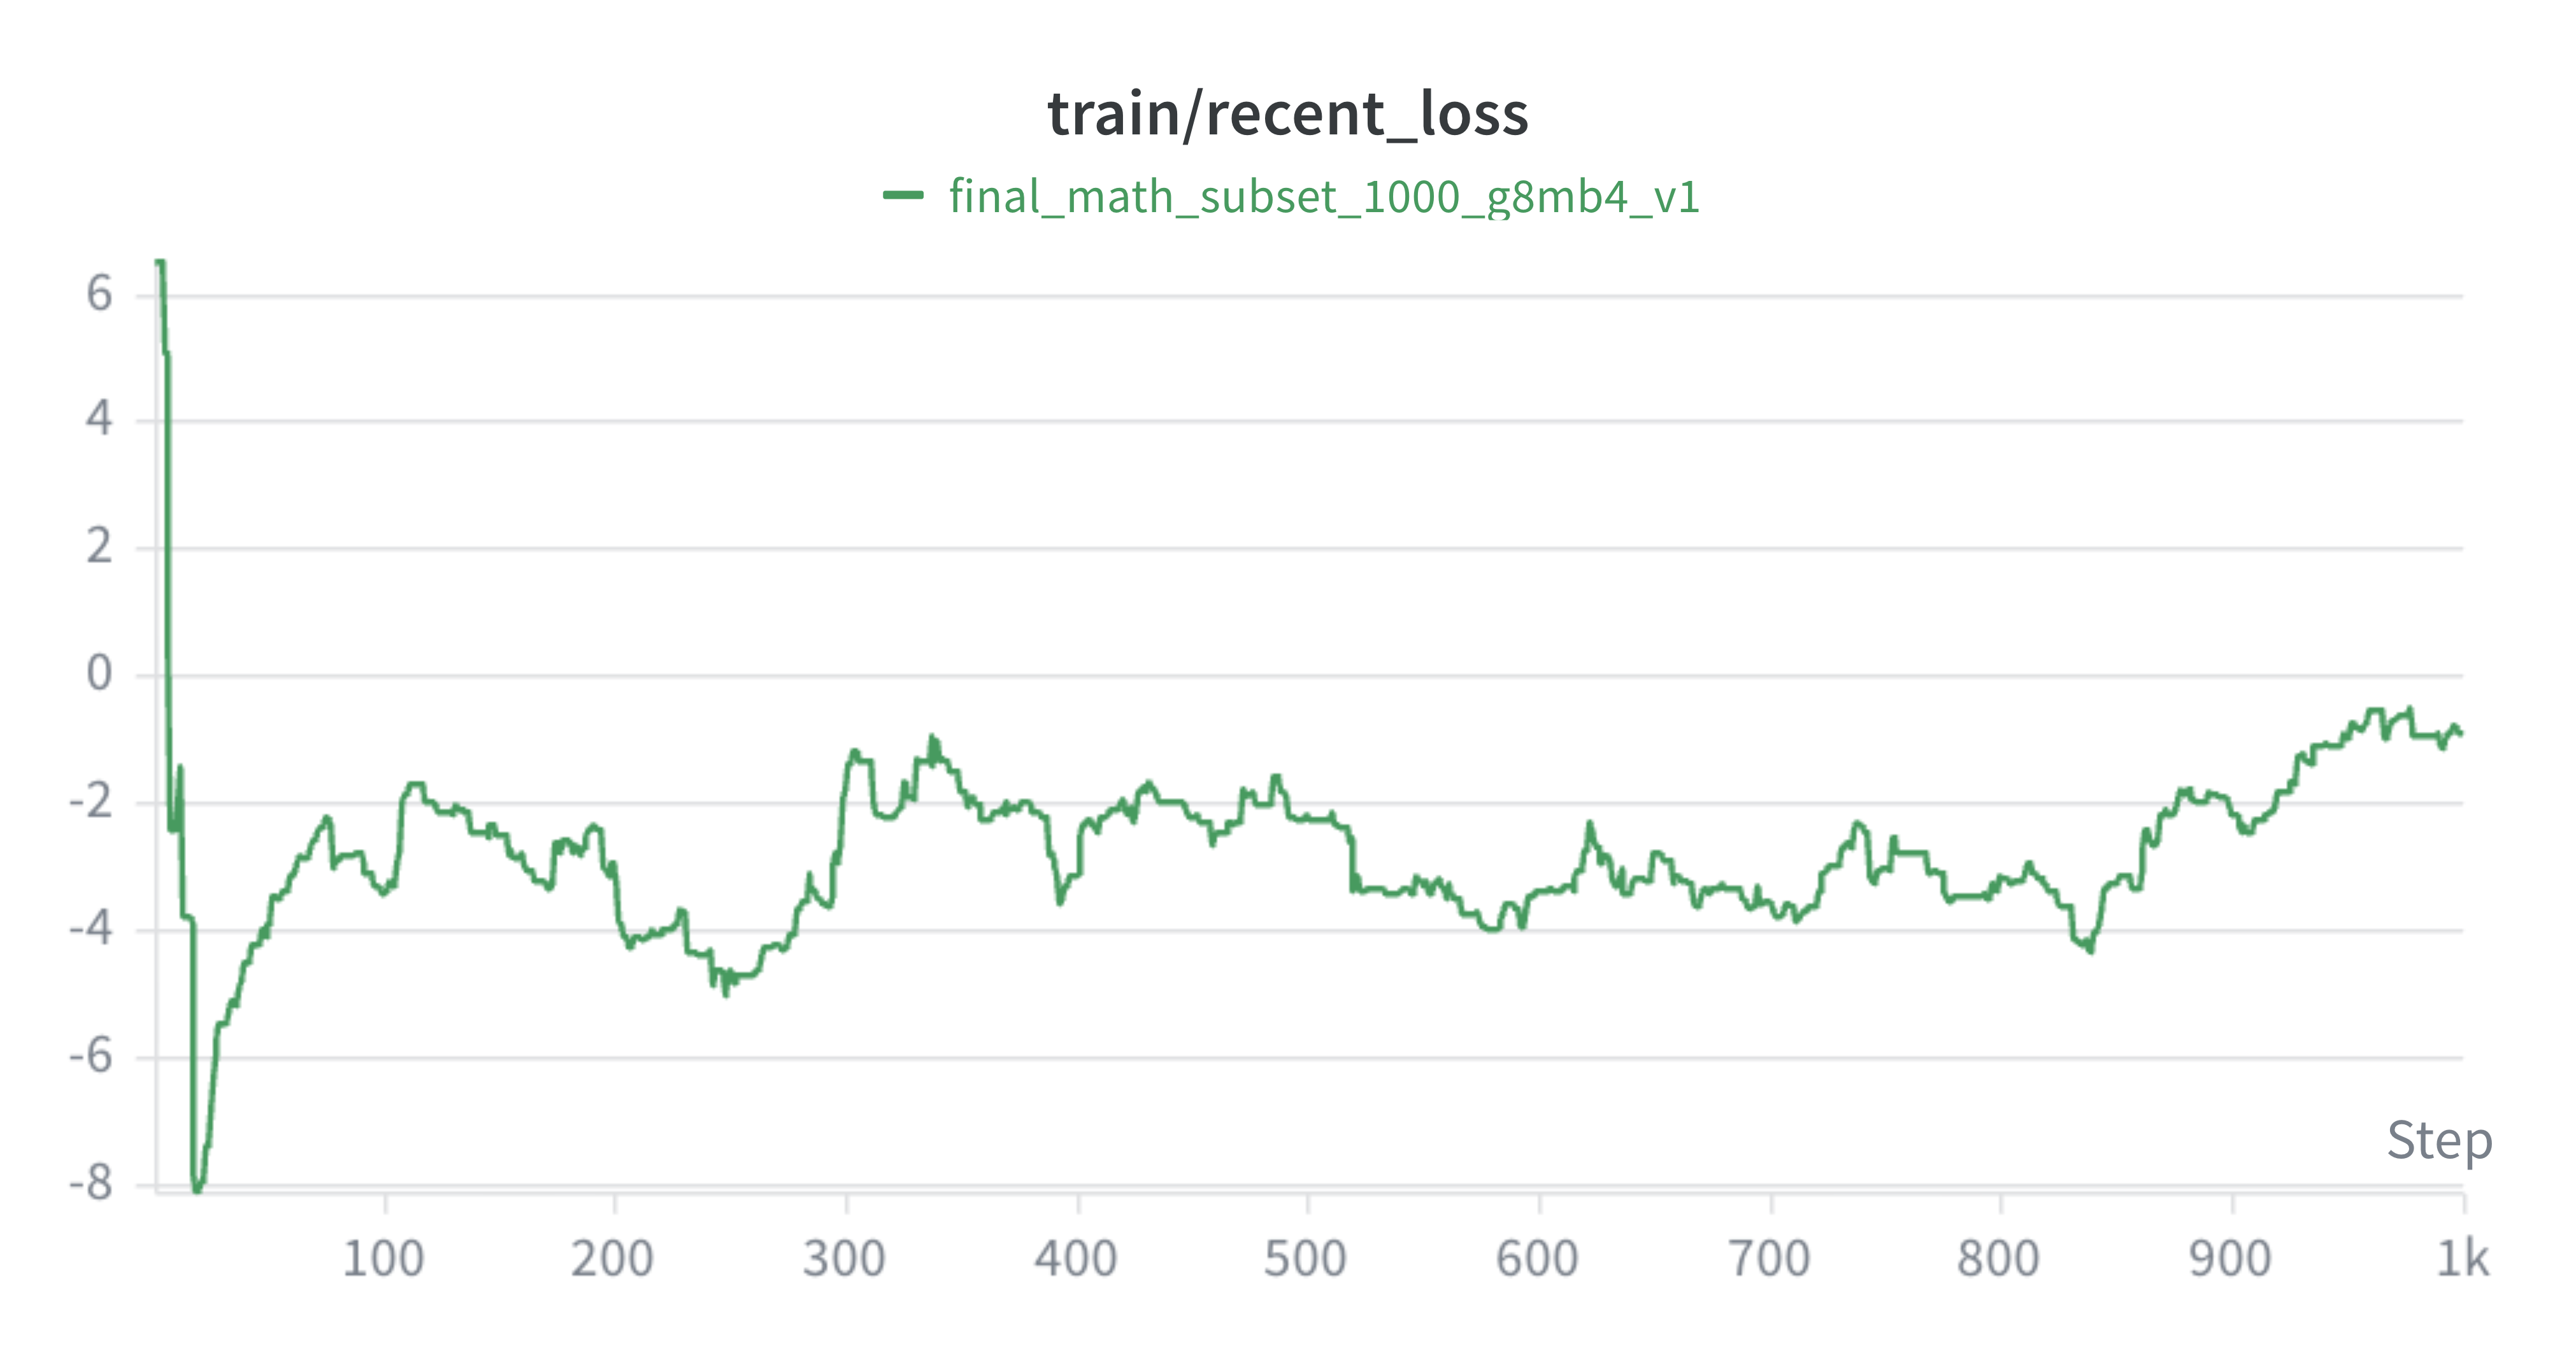
\includegraphics[width=\linewidth]{math_train_recent_loss.png}
    \caption{Policy loss.}
  \end{subfigure}
  \caption{Additional training signals for the GRPO run on the math-specialized base (Section~\ref{sec:math-base}). Rolling accuracy oscillates with no upward trend; reward and loss show no meaningful improvement over the run, consistent with the zero-gradient regime diagnosed in the main text.}
  \label{fig:app-math}
\end{figure}

\subsection{DAPO on the Math-Specialized Base}
\label{app:dapo}

\begin{figure}[H]
  \centering
  \begin{subfigure}{0.32\textwidth}
    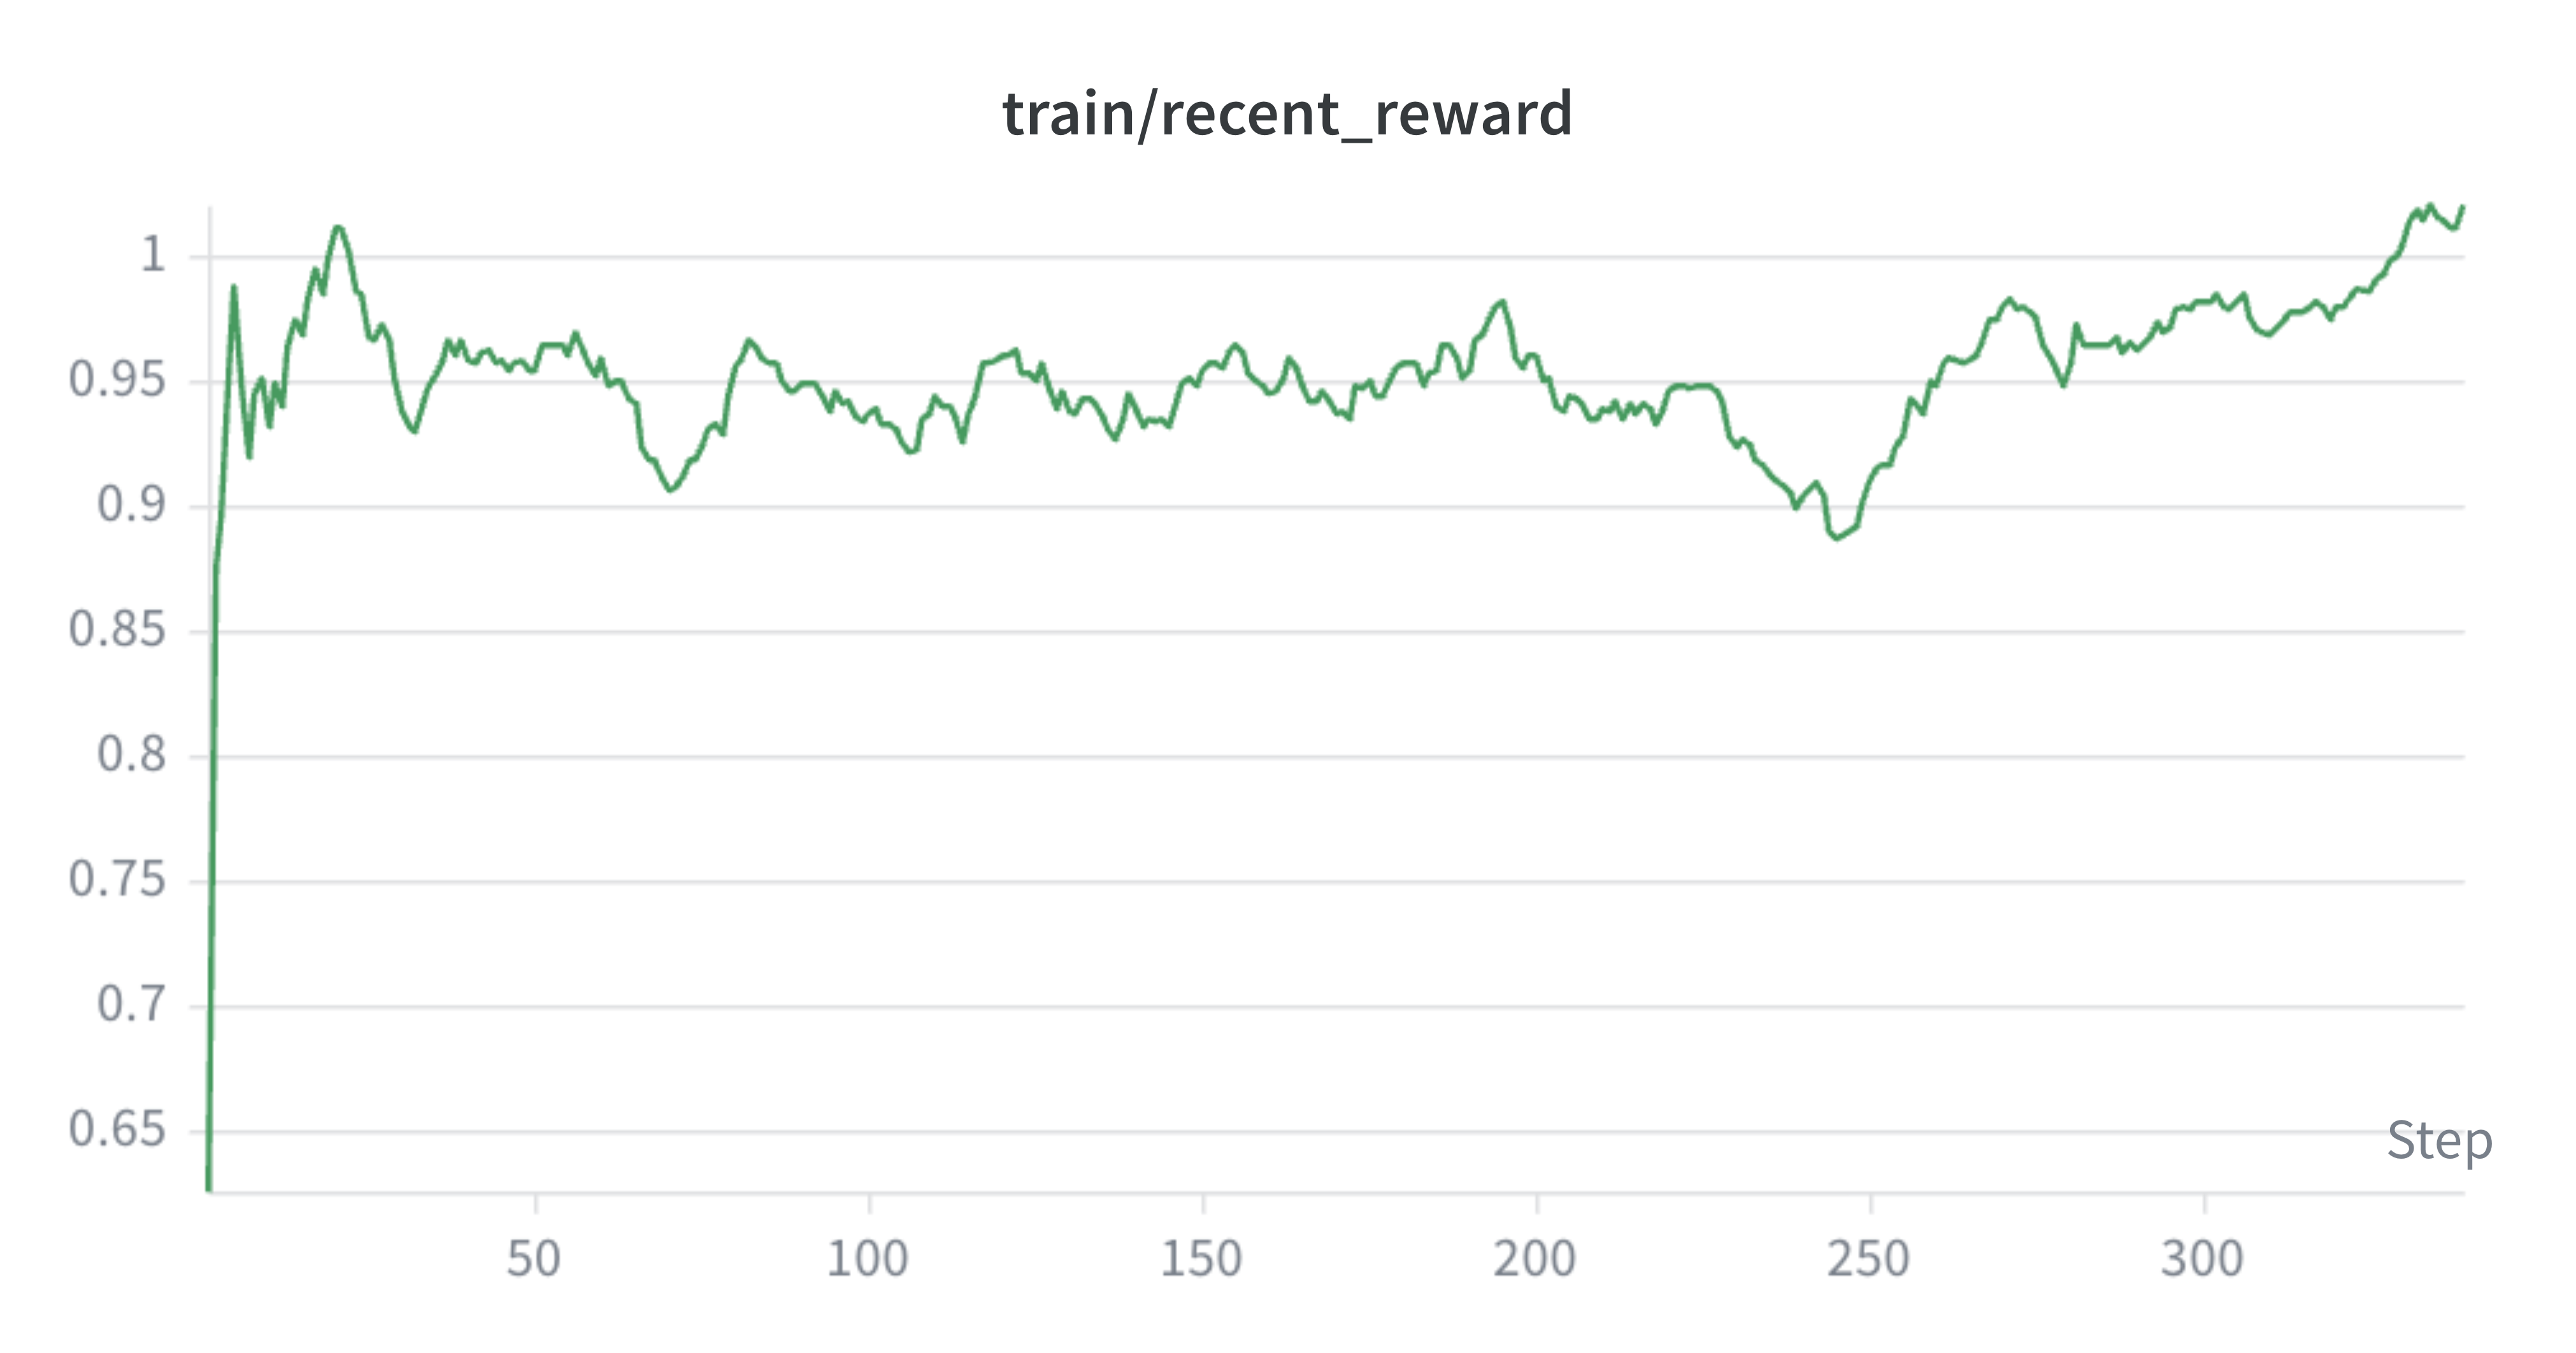
\includegraphics[width=\linewidth]{dapo_train_recent_reward.png}
    \caption{Rolling reward.}
  \end{subfigure}
  \hfill
  \begin{subfigure}{0.32\textwidth}
    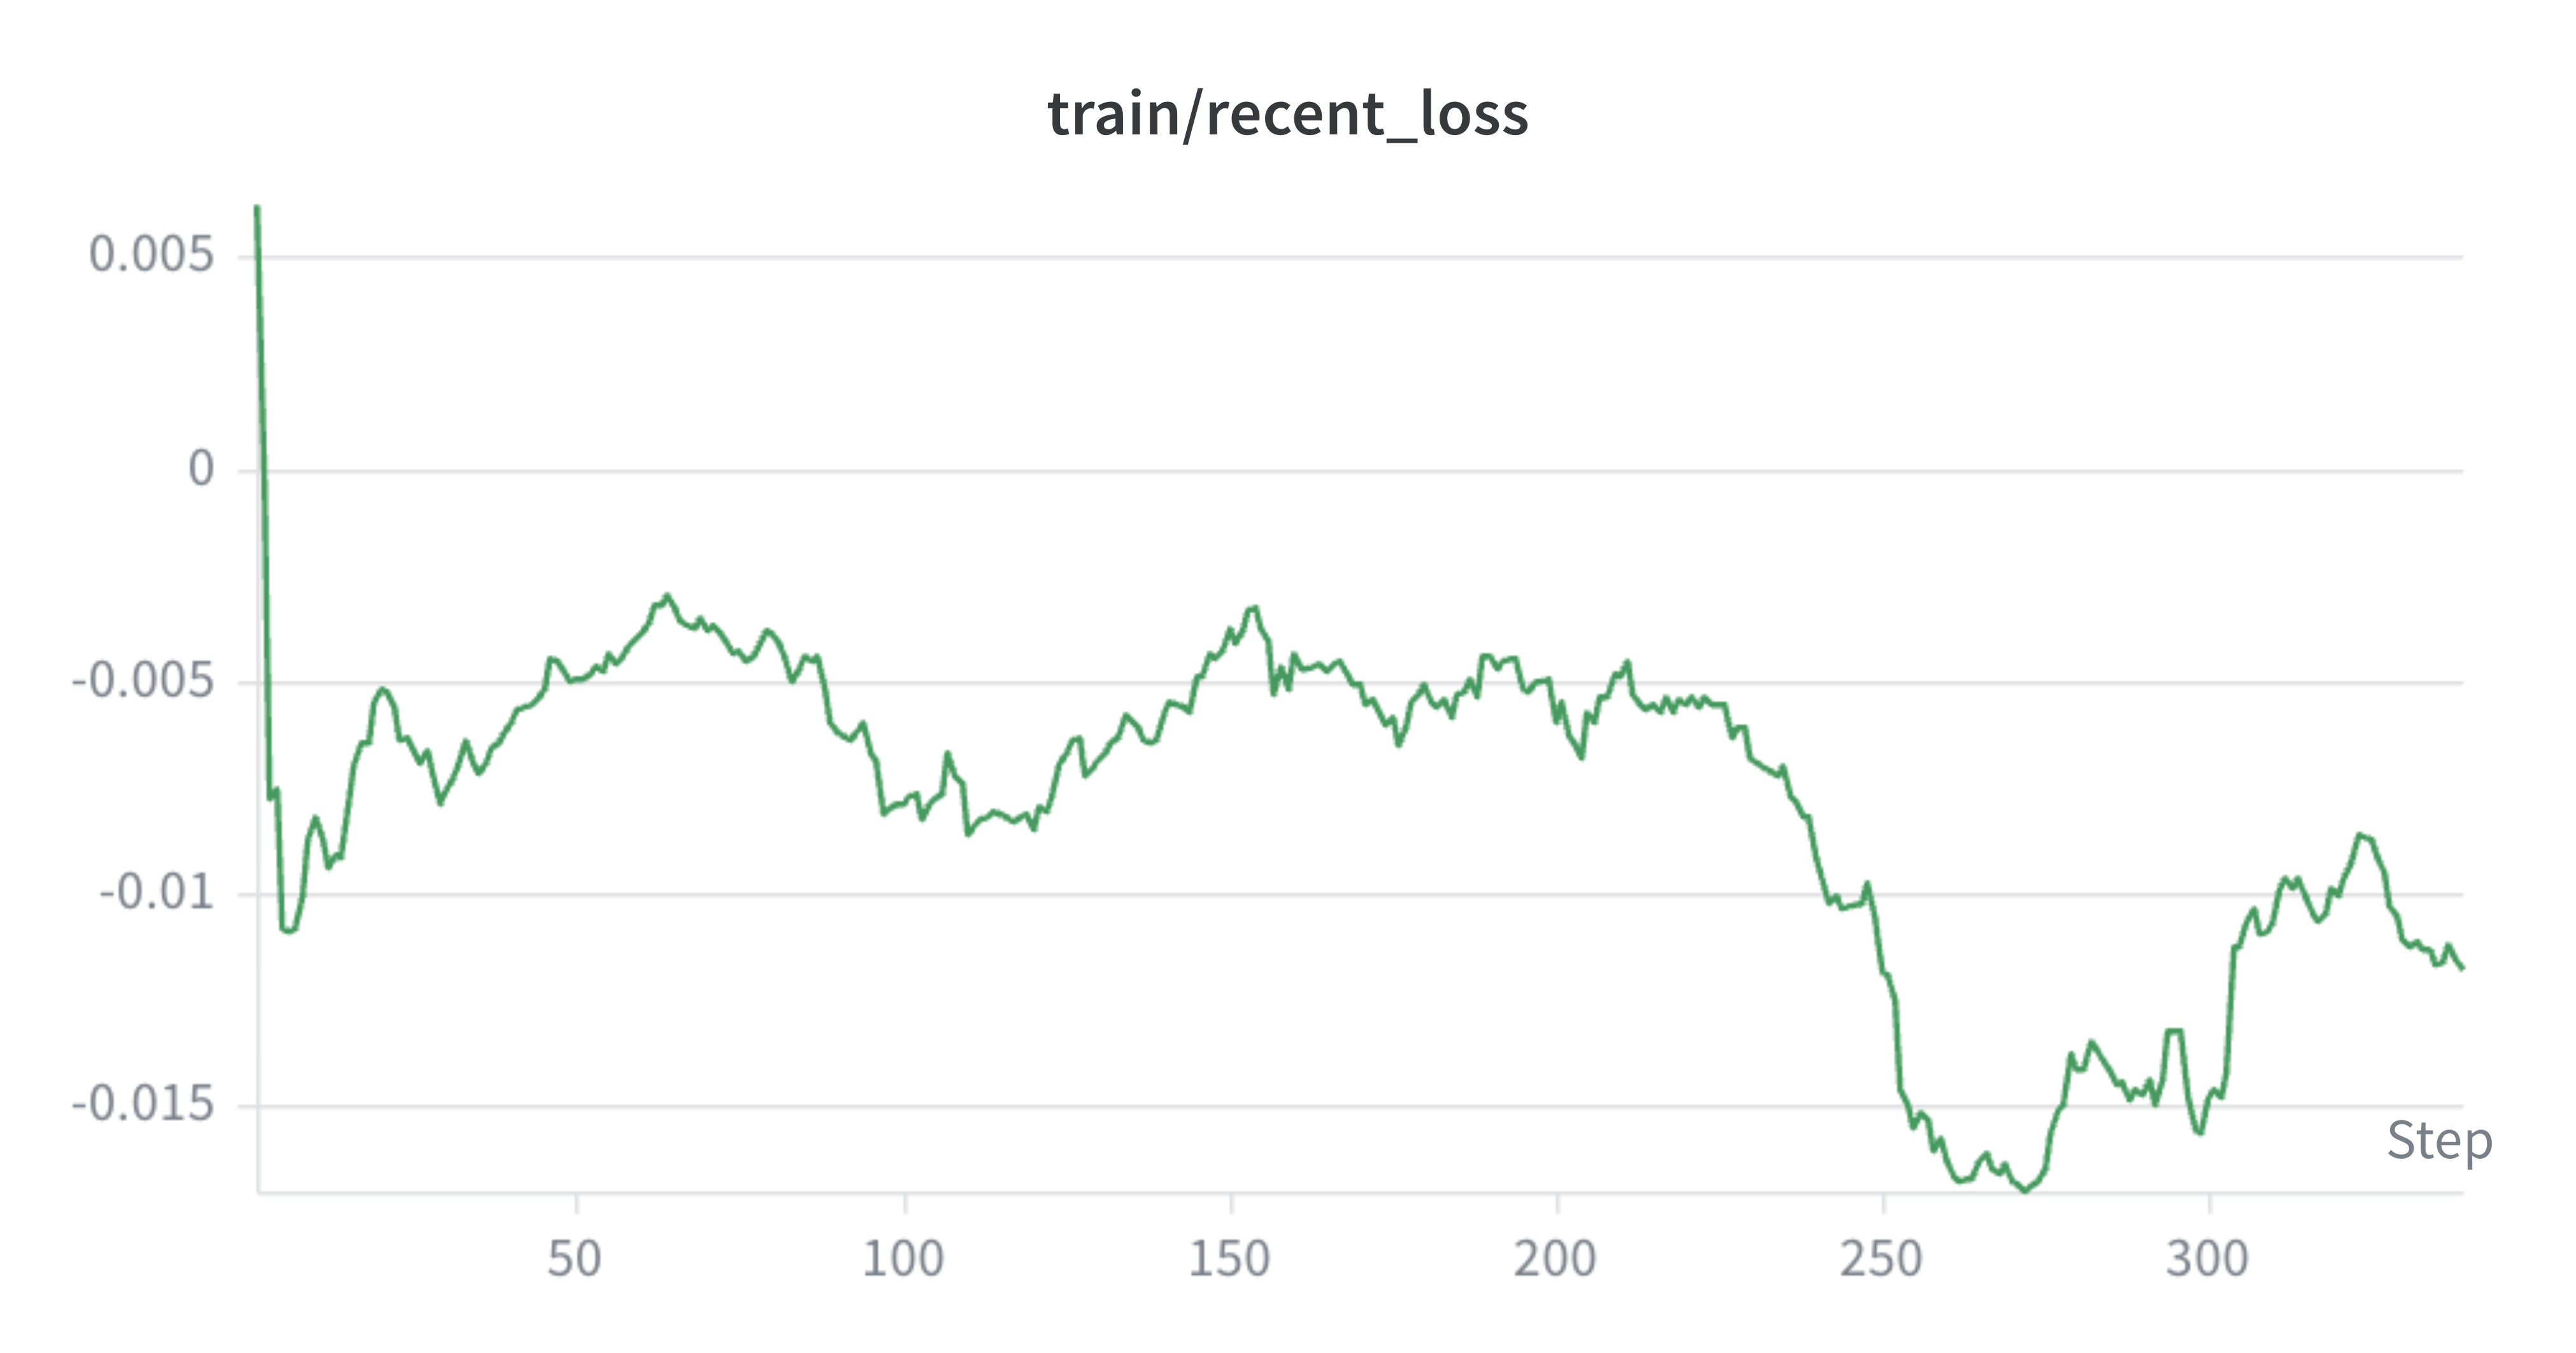
\includegraphics[width=\linewidth]{dapo_train_recent_loss.png}
    \caption{Policy loss.}
  \end{subfigure}
  \hfill
  \begin{subfigure}{0.32\textwidth}
    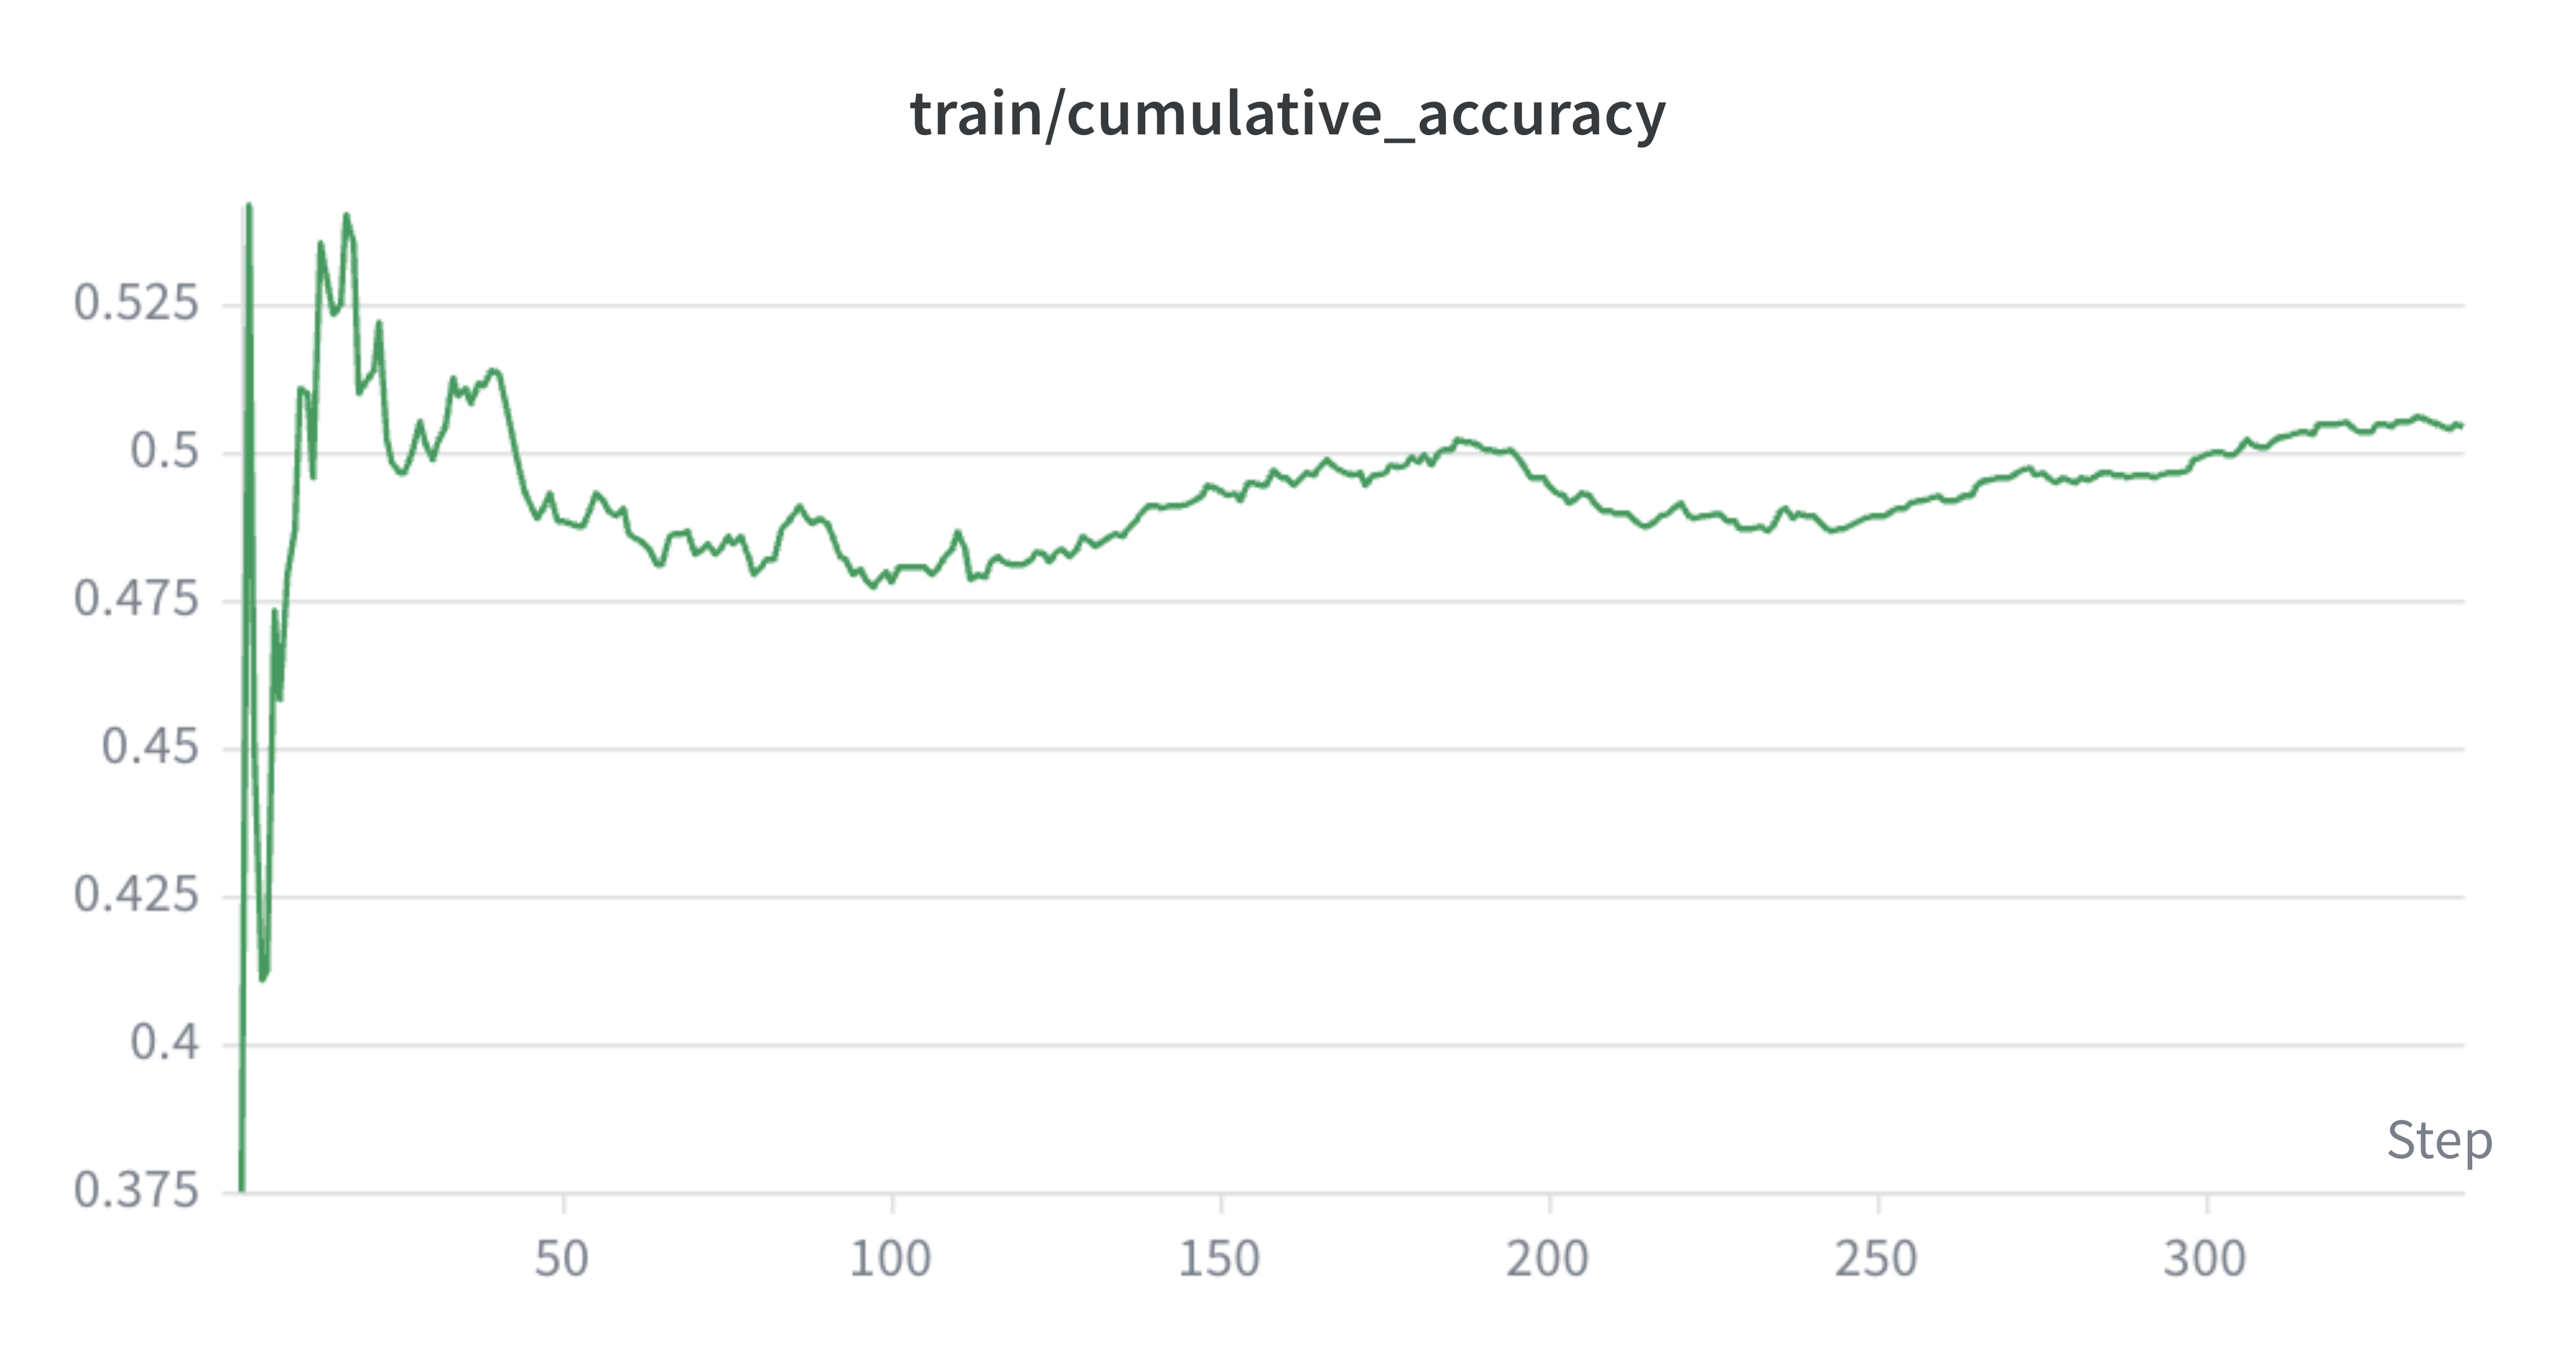
\includegraphics[width=\linewidth]{dapo_train_cumulative_accuracy.png}
    \caption{Cumulative accuracy.}
  \end{subfigure}
  \caption{Additional training signals for the DAPO run (Section~\ref{sec:dapo}). Per-step reward rises from $\sim$0.65 to $\sim$1.01, policy loss trends toward $-$0.016, and cumulative accuracy on the filtered \texttt{mixed\_hard} training subset stabilizes near 50\%---the expected level for questions the base model cannot solve consistently.}
  \label{fig:app-dapo}
\end{figure}

\newpage
\begin{thebibliography}{99}

\bibitem[Yu et~al.(2025)]{yu2025dapo}
    Qiying Yu et~al.
    \newblock \emph{DAPO: An Open-Source LLM Reinforcement Learning System at Scale}.
    \newblock arXiv:2503.14476, 2025.
    \newblock \url{https://arxiv.org/abs/2503.14476}.

\bibitem[Cobbe et~al.(2021)]{cobbe2021}
Karl Cobbe, Vineet Kosaraju, Mohammad Bavarian, Mark Chen, Heewoo Jun, Lukasz Kaiser, Matthias Plappert, Jerry Tworek, Jacob Hilton, Reiichiro Nakano, Christopher Hesse, and John Schulman.
\newblock \emph{Training Verifiers to Solve Math Word Problems}.
\newblock arXiv:2110.14168, 2021.
\newblock \url{https://arxiv.org/abs/2110.14168}.

\bibitem[DeepSeek-AI(2025)]{deepseekr1}
DeepSeek-AI.
\newblock \emph{DeepSeek-R1: Incentivizing Reasoning Capability in LLMs via Reinforcement Learning}.
\newblock arXiv:2501.12948, 2025.
\newblock \url{https://arxiv.org/abs/2501.12948}.

\bibitem[Hu et~al.(2021)]{hu2021lora}
Edward~J. Hu, Yelong Shen, Phillip Wallis, Zeyuan Allen-Zhu, Yuanzhi Li, Shean Wang, Lu Wang, and Weizhu Chen.
\newblock \emph{LoRA: Low-Rank Adaptation of Large Language Models}.
\newblock arXiv:2106.09685, 2021.
\newblock \url{https://arxiv.org/abs/2106.09685}.

\bibitem[Lambert et~al.(2024)]{lambert2024tulu3}
Nathan Lambert et~al.
\newblock \emph{T\"ulu 3: Pushing Frontiers in Open Language Model Post-Training}.
\newblock arXiv:2411.15124, 2024.
\newblock \url{https://arxiv.org/abs/2411.15124}.

\bibitem[Lightman et~al.(2023)]{lightman2023verify}
Hunter Lightman, Vineet Kosaraju, Yura Burda, Harri Edwards, Bowen Baker, Teddy Lee, Jan Leike, John Schulman, Ilya Sutskever, and Karl Cobbe.
\newblock \emph{Let's Verify Step by Step}.
\newblock arXiv:2305.20050, 2023.
\newblock \url{https://arxiv.org/abs/2305.20050}.

\bibitem[Ouyang et~al.(2022)]{ouyang2022instructgpt}
Long Ouyang, Jeff Wu, Xu Jiang, Diogo Almeida, Carroll~L. Wainwright, Pamela Mishkin, Chong Zhang, Sandhini Agarwal, Katarina Slama, Alex Ray, John Schulman, Jacob Hilton, Fraser Kelton, Luke Miller, Maddie Simens, Amanda Askell, Peter Welinder, Paul Christiano, Jan Leike, and Ryan Lowe.
\newblock \emph{Training Language Models to Follow Instructions with Human Feedback}.
\newblock arXiv:2203.02155, 2022.
\newblock \url{https://arxiv.org/abs/2203.02155}.

\bibitem[Schulman et~al.(2017)]{schulman2017ppo}
John Schulman, Filip Wolski, Prafulla Dhariwal, Alec Radford, and Oleg Klimov.
\newblock \emph{Proximal Policy Optimization Algorithms}.
\newblock arXiv:1707.06347, 2017.
\newblock \url{https://arxiv.org/abs/1707.06347}.

\bibitem[Shao et~al.(2024)]{shao2024deepseekmath}
Zhihong Shao, Peiyi Wang, Qihao Zhu, Runxin Xu, Junxiao Song, Xiao Bi, Haowei Zhang, Mingchuan Zhang, Y.~K. Li, Y. Wu, and Daya Guo.
\newblock \emph{DeepSeekMath: Pushing the Limits of Mathematical Reasoning in Open Language Models}.
\newblock arXiv:2402.03300, 2024.
\newblock \url{https://arxiv.org/abs/2402.03300}.

\bibitem[Wang et~al.(2022)]{wang2022sc}
Xuezhi Wang, Jason Wei, Dale Schuurmans, Quoc Le, Ed~H. Chi, Sharan Narang, Aakanksha Chowdhery, and Denny Zhou.
\newblock \emph{Self-Consistency Improves Chain of Thought Reasoning in Language Models}.
\newblock arXiv:2203.11171, 2022.
\newblock \url{https://arxiv.org/abs/2203.11171}.

\bibitem[Wei et~al.(2022)]{wei2022cot}
Jason Wei, Xuezhi Wang, Dale Schuurmans, Maarten Bosma, Brian Ichter, Fei Xia, Ed~H. Chi, Quoc Le, and Denny Zhou.
\newblock \emph{Chain-of-Thought Prompting Elicits Reasoning in Large Language Models}.
\newblock arXiv:2201.11903, 2022.
\newblock \url{https://arxiv.org/abs/2201.11903}.

\bibitem[Yang et~al.(2024)]{yang2024qwen25math}
An Yang, Beichen Zhang, Binyuan Hui, Bofei Gao, Bowen Yu, Chengpeng Li, Dayiheng Liu, Jianhong Tu, Jingren Zhou, Junyang Lin, Keming Lu, Mingfeng Xue, Runji Lin, Tianyu Liu, Xingzhang Ren, and Zhenru Zhang.
\newblock \emph{Qwen2.5-Math Technical Report: Toward Mathematical Expert Model via Self-Improvement}.
\newblock arXiv:2409.12122, 2024.
\newblock \url{https://arxiv.org/abs/2409.12122}.

\bibitem[Yao et~al.(2022)]{yao2022react}
Shunyu Yao, Jeffrey Zhao, Dian Yu, Nan Du, Izhak Shafran, Karthik Narasimhan, and Yuan Cao.
\newblock \emph{ReAct: Synergizing Reasoning and Acting in Language Models}.
\newblock arXiv:2210.03629, 2022.
\newblock \url{https://arxiv.org/abs/2210.03629}.

\end{thebibliography}

\end{document}
